% Copyright (c) 2015 Daniele Masini - d.masini.it@gmail.com
% Copyright (c) 2016 Daniele Zambelli - daniele.zambelli@gmail.com

\chapter{Rette parallele}
\label{chap:rette_parallele}

\includegraphics[width=0.95\textwidth]
  {\folder img/intersection_de_deux_paralleles.jpg}
  \begin{center}
    {\large ``Intersection de deux parallèles''}\par
    Foto di OliBac\par
    \url{http://www.flickr.com/photos/olibac/3244014009/}\par
    Licenza: Creative Commons Attribution\par
  \end{center}
\newpage

\section{Primo teorema dell'angolo 
esterno}\label{sect:primo_teorema_angolo_esterno}

Ricordiamo che un angolo esterno di un poligono è un angolo che ha 
come vertice un vertice del poligono ed è adiacente ad un angolo 
interno.

\begin{teorema}[dell'angolo esterno]
In un triangolo, un angolo esterno è maggiore di ciascuno dei due 
angoli interni non adiacenti.
\end{teorema}


\begin{inaccessibleblock}[Figura: TODO]
 \begin{figure}[htb]
\centering% Copyright (c) 2015 Daniele Masini - d.masini.it@gmail.com

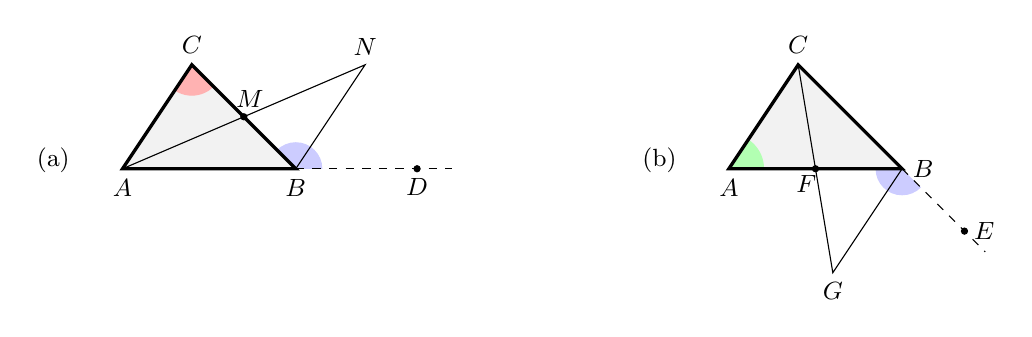
\begin{tikzpicture}[scale=1.1,font=\small]
\usetikzlibrary{calc}

\begin{scope}

\coordinate (a) at (0,0);
\coordinate (c) at (0.8,1.2);
\coordinate (b) at (2,0);

\draw[fill,gray!10] (a) -- (b) -- (c);

\draw[fill] ($(a)!1.7!(b)$) circle(1pt) coordinate (d) node[below] {$D$};

\begin{scope}
\clip (a) -- (b) -- (c) -- cycle;
\draw[fill,red!30] (c) circle (0.35);
\end{scope}

\begin{scope}
\clip (c) -- (b) -- (d) -- cycle;
\draw[fill,blue!20] (b) circle (0.3);
\end{scope}

\draw[very thick] (a) node[below] {$A$} -- (b) node[below] {$B$} -- (c) node[above] {$C$} -- cycle;
\draw[dashed] (b) -- ($(a)!1.9!(b)$);
\coordinate (m) at ($(b)!0.5!(c)$);
\draw (a) -- ($(a)!2!(m)$) coordinate (n) node[above] {$N$} -- (b);
\draw[fill] (m) circle (1pt);
\path ([shift={(2pt,6pt)}]m) node {$M$};

\node at (-.8,0.1) {(a)};

\end{scope}

\begin{scope}[xshift=7cm]

\coordinate (a) at (0,0);
\coordinate (c) at (0.8,1.2);
\coordinate (b) at (2,0);

\draw[fill,gray!10] (a) -- (b) -- (c);

\draw[fill] ($(c)!1.6!(b)$) circle(1pt) coordinate (e) node[right] {$E$};

\begin{scope}
\clip (a) -- (b) -- (c) -- cycle;
\draw[fill,green!30] (a) circle (0.4);
\end{scope}

\begin{scope}
\clip (a) -- (b) -- (e) -- cycle;
\draw[fill,blue!20] (b) circle (0.3);
\end{scope}

\draw[very thick] (a) node[below] {$A$} -- (b) node[right] {$B$} -- (c) node[above] {$C$} -- cycle;
\draw[dashed] (b) -- ($(c)!1.8!(b)$);
\coordinate (f) at ($(a)!0.5!(b)$);
\draw (c) -- ($(c)!2!(f)$) coordinate (g) node[below] {$G$} -- (b);
\draw[fill] (f) circle (1pt);
\path ([shift={(-3pt,-5pt)}]f) node {$F$};

\node at (-.8,0.1) {(b)};

\end{scope}


\end{tikzpicture}

\end{figure}
\end{inaccessibleblock}

\begin{proof}
Sia $ABC$ un triangolo (figura~a). Prolunghiamo il lato $AB$ dalla 
parte di $B$ e prendiamo un qualsiasi punto $D$ sul prolungamento. 
Vogliamo dimostrare che l'angolo $C\widehat{B}D$ è maggiore sia 
dell'angolo $C\widehat{A}B$ sia dell'angolo $A\widehat{C}B$. A tal 
fine prendiamo il punto medio del lato $CB$, lo chiamiamo $M$; uniamo 
$A$ con $M$ e prolunghiamo $AM$ dalla parte di $M$, prendendo un 
punto $N$ sul prolungamento in modo che $AM$ sia congruente a $MN$; 
uniamo $N$ con $B$.

Osserviamo che i triangoli $AMC$ e $BNM$ sono congruenti per il primo 
criterio, infatti: $CM\cong MB$ perché $M$ è un punto medio per 
costruzione, $AM\cong MN$ per costruzione e $C\widehat{M}A\cong 
B\widehat{M}N$ perché opposti al vertice.
Di conseguenza i restanti elementi dei due triangoli sono 
ordinatamente congruenti, in particolare $A\widehat{C}M\cong 
M\widehat{B}N$. Ma l'angolo $M\widehat{B}N$ è una parte propria 
dell'angolo esterno $C\widehat{B}D$ che risulta pertanto maggiore di 
$M\widehat{B}N$ e dell'angolo interno di vertice $C$.

Rimane ora da dimostrare che $C\widehat{B}D$ è anche maggiore di 
$C\widehat{A}B$ ma per farlo occorre un'altra costruzione (figura~b).
Prolunghiamo il segmento $CB$ dalla parte di $B$ viene individuato un 
altro angolo esterno $A\widehat{B}E$, che però è congruente al 
precedente: è anch'esso adiacente all'angolo interno di vertice $B$ 
ed è opposto al vertice di $C\widehat{B}D$. Usiamo tale angolo ed una 
costruzione analoga alla precedente a partire dal punto medio $F$ del 
segmento $AB$ e dal punto $G$ sul prolungamento di $CF$, con $CF\cong 
FG$, in modo da ottenere, dal confronto dei triangoli congruenti 
$AFC$ e $FGB$, che l'angolo interno di vertice $A$ è congruente 
all'angolo $F\widehat{B}G$ che è una parte propria dell'angolo esterno 
di vertice $B$, $A\widehat{B}E\cong C\widehat{B}D$.
\end{proof}

\section{Rette perpendicolari}\label{sect:rette_perpendicolari}

Ricordiamo che due rette giacenti su uno stesso piano si dicono 
\emph{perpendicolari} se si incontrano dividendo il piano in quattro 
angoli congruenti. In realtà è sufficiente sapere che uno dei quattro 
angoli che si vengono a formare è retto, per concludere che sono 
tutti retti.

\begin{proprieta}
Siano $AB$ e $CD$ due rette incidenti di intersezione $E$, se risulta 
che l'angolo $A\widehat{E}C$ è retto, allora sono retti anche gli 
angoli $A\widehat{E}D$, $B\widehat{E}C$ e $B\widehat{E}D$.
\end{proprieta}

\noindent\begin{minipage}{.65\textwidth}
\begin{proof}~\\
L'angolo $A\widehat{E}D$ è retto perché adiacente all'angolo retto 
$A\widehat{E}C$.\\
L'angolo $D\widehat{E}B$ è retto perché opposto al vertice all'angolo 
retto $A\widehat{E}C$.\\
L'angolo $C\widehat{E}B$ è retto perché adiacente all'angolo retto 
$A\widehat{E}C$.
\end{proof}
\end{minipage}\hfil
\begin{minipage}{.35\textwidth}
\centering% Copyright (c) 2015 Daniele Masini - d.masini.it@gmail.com

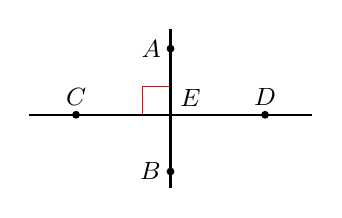
\begin{tikzpicture}[scale=1.2,font=\small]
\usetikzlibrary{calc}

\begin{scope}

\coordinate (a) at (0,.7);
\coordinate (c) at (-1,0);
\coordinate (b) at (0,-0.6);
\coordinate (d) at (1,0);
\coordinate (e) at (0,0);

\draw[red] (-0.3,0) rectangle (0,0.3);

\draw[thick] ($(c)!-0.5!(e)$) -- ($(e)!1.5!(d)$);
\draw[thick] ($(b)!-0.3!(e)$) -- ($(e)!1.3!(a)$);

\draw[fill] (a) circle (1pt) node[left] {$A$};
\draw[fill] (b) circle (1pt) node[left] {$B$};
\draw[fill] (c) circle (1pt) node[above] {$C$};
\draw[fill] (d) circle (1pt) node[above] {$D$};
\draw (e) node[above=6pt, right] {$E$};

\end{scope}

\end{tikzpicture}

\end{minipage}
~\\

Quindi, se due rette incidenti formano un angolo retto allora tutti 
gli angoli che si formano sono retti.

L'esistenza e l'unicità della perpendicolare sono assicurate dal 
seguente teorema.

\begin{teorema}
Nel piano, data una retta ed un punto, esiste ed è unica la retta 
perpendicolare alla retta data e passante per il punto assegnato.
\end{teorema}


\begin{inaccessibleblock}[Figura: TODO]
 \begin{figure}[htb]
\centering% Copyright (c) 2015 Daniele Masini - d.masini.it@gmail.com

\begin{tikzpicture}[scale=1.2,font=\small, dot/.style={circle,inner sep=1pt, fill, label={#1}, name=#1}, extended line/.style={shorten >=-#1,shorten <=-#1}, extended line/.default=1cm]
\usetikzlibrary{calc, intersections}

\begin{scope}

\coordinate (c) at (0,1);
\coordinate (a) at (-1,0);
\coordinate (d) at (0,-1);
\coordinate (b) at (1,0);
\coordinate (p) at (0,0);
\coordinate (e) at (0.5,1);

%\draw[red] (-0.3,0) rectangle (0,0.3);
\draw[blue, dashed] ($(e)!-0.3!(p)$) -- ($(e)!2.3!(p)$);
\draw[fill] (e) circle (1pt) node[right] {$E$};

\draw[blue, extended line=0.5cm] (c) -- (d);
\draw[thick, extended line=0.5cm] (a) -- (b);

\draw[fill] (a) circle (1pt) node[above] {$A$};
\draw[fill] (b) circle (1pt) node[above] {$B$};
\draw[fill] (c) circle (1pt) node[left] {$C$};
\draw[fill] (d) circle (1pt) node[right] {$D$};
\draw[fill] (p) circle (1pt) node[above=6pt, left] {$P$};

\node at (0,-2) {(a)};

\end{scope}


\begin{scope}[xshift=5cm]

\coordinate (p) at (0,1);
\coordinate (a) at (-1.5,0);
\coordinate (t) at (0,-1);
\coordinate (b) at (1.5,0);
\coordinate (e) at (0.5,1);
\coordinate (q) at (-0.6,0);
\coordinate (r) at ($(q)!1.4!(t)$);

%\draw [extended line] ($(a)!(p)!(b)$) -- (p);

\draw[thick, extended line=0.5cm] (a)--(b);

\draw[fill] (a) circle (1pt) node[above] {$A$};
\draw[fill] (b) circle (1pt) node[above] {$B$};
\draw[fill] (c) circle (1pt) node[left] {$C$};
\draw[fill] (t) circle (1pt) node[right] {$T$};
\draw[fill] (q) circle (1pt) node[below=7pt, left] {$Q$};
\draw[fill] (p) circle (1pt) node[above] {$P$};
\draw[fill] (r) circle (1pt) node[right] {$R$};

\draw (q) -- (p);
\draw (q) -- ($(q)!1.2!(r)$);
\draw[blue] (t) -- (p);
\coordinate (h) at (intersection of t--p and a--b);
\draw[fill] (h) circle (1pt) node[below=7pt, right] {$H$};

\node at (0,-2) {(b)};

\end{scope}

\end{tikzpicture}

\end{figure}
\end{inaccessibleblock}

\begin{proof}
Per la dimostrazione, distinguiamo due casi.

Primo caso: il punto appartiene alla retta (figura~a).
Sia $AB$ una retta del piano e sia $P$ un suo punto. Allora se 
tracciamo la bisettrice dell'angolo piatto $A\widehat{P}B$, questa è 
certamente perpendicolare ad $AB$, in quanto i due angoli che si 
vengono a formare sono retti.
Prolungando questa bisettrice, si viene a formare una retta $CD$ 
perpendicolare ad $AB$.  
Supponiamo per assurdo che la retta $CD$ non sia l'unica 
perpendicolare ad $AB$ passante per il punto $P$ ma che ne esista 
un'altra. Detto $E$ un punto su tale ipotetica retta distinto da $P$, 
se $E$ appartenesse anche alla retta $CD$, allora $PE$ coinciderebbe 
con $CD$, quindi $PE$ non sarebbe distinta dalla retta $CD$; se 
invece $E$ non appartenesse a $CD$, unendo $E$ con $P$ si verrebbero 
a formare due angoli $A\widehat{P}E$ e $E\widehat{P}B$ di cui uno 
acuto ed uno ottuso e quindi la retta $EP$ non risulterebbe 
perpendicolare ad $AB$.

Secondo caso: il punto non appartiene alla retta (figura~b).
Sia $AB$ una retta nel piano e sia $P$ un punto del piano non 
appartenente ad essa. Costruiamo la perpendicolare ad $AB$ passante 
per $P$ e dimostriamo che è unica.
Possiamo prendere un punto $Q$ appartenente ad $AB$ e congiungere $P$ 
con $Q$. Se gli angoli $A\widehat{Q}P$ e $P\widehat{Q}B$ sono retti, 
abbiamo già trovato la perpendicolare. Altrimenti, vuol dire che gli 
angoli $A\widehat{Q}P$ e $P\widehat{Q}B$ sono uno acuto ed uno 
ottuso. Tracciamo la semiretta $QR$, di origine $Q$ e giacente nel 
semipiano individuato da $AB$ non contenente il punto $P$: essa lo 
divide in due angoli, $A\widehat{Q}R$ e $R\widehat{Q}B$, 
rispettivamente congruenti a $A\widehat{Q}P$ e $P\widehat{Q}B$. 
Prendiamo un punto $T$ su tale semiretta in modo che $QT\cong QP$. 
Uniamo $P$ con $T$ e chiamiamo $H$ il punto di intersezione tra $PT$ 
ed $AB$. Allora il triangolo $QPT$ è isoscele sulla base $PT$ e il 
segmento $QH$ è la bisettrice dell'angolo al vertice $P\widehat{Q}T$, 
che risulta pertanto essere anche mediana ed altezza relativa alla 
base $PT$. Dunque gli angoli $P\widehat{H}Q$ e $T\widehat{H}Q$ sono 
retti e quindi la retta $PT$ è perpendicolare ad $AB$.
Abbiamo quindi trovato la perpendicolare ad $AB$ passante per $P$. 
Per dimostrare che è unica possiamo ricorrere al ragionamento fatto 
nel primo caso, dove ora $H$ è il punto $P$ della dimostrazione 
precedente.

Il teorema è pertanto dimostrato.
\end{proof}

\section{Rette parallele}\label{sect:rette_parallele}

Secondo la definizione di Euclide, due rette nel piano sono parallele 
se non hanno punti in comune.
In maniera più moderna il concetto di parallelismo è interpretato 
come l'avere la stessa direzione.
Si può anche dare una formulazione che unifichi le due definizioni 
precedenti; si deve però ricorrere al concetto di distanza: due rette 
nel piano sono parallele se mantengono sempre la stessa distanza. Se 
la distanza è nulla, le due rette sono coincidenti.
Noi utilizzeremo la seguente:
\begin{definizione}
Due rette giacenti nello stesso piano si dicono \emph{parallele} se 
sono coincidenti oppure non si incontrano mai.
\end{definizione}

Assumendo dunque questa come definizione di parallelismo, abbiamo 
bisogno di precisare il concetto di distanza.
Dati due punti $P$ e $Q$, la \emph{distanza} tra $P$ e $Q$ è la 
lunghezza del \emph{percorso più breve} che unisce i due punti. 
Questo concetto è valido anche se si riferisce alle distanze tra due 
città che si trovano negli stradari: sono riportate le lunghezze dei 
percorsi minimi tra tutte le strade alternative che collegano due 
città. Naturalmente, nel piano, ove si ``dispone'' di tutti i punti 
da poter ``attraversare'', il percorso più breve che collega due 
punti $P$ e $Q$ è il segmento $PQ$; quindi nella geometria euclidea 
assumiamo come distanza tra due punti la lunghezza del segmento 
avente per estremi i due punti.

Se vogliamo parlare di distanza tra due insiemi di punti, allora va 
considerato il percorso più breve tra tutti i percorsi che collegano 
un qualsiasi punto del primo insieme con un qualsiasi punto del 
secondo: in pratica la distanza è la lunghezza del più piccolo 
segmento tra tutti quelli che collegano i due insiemi di punti. 

Nel caso particolare di un punto $A$ ed una retta $BC$, se il punto 
appartiene alla retta allora la distanza di $A$ da $BC$ è uguale a 
zero, altrimenti si considera come distanza la lunghezza del segmento 
$AH$, dove $H$ è il punto in cui la perpendicolare a $BC$ passante 
per $A$ interseca la stessa retta $BC$: il motivo si intuisce in base 
a quanto detto, ma risulterà chiaro più avanti, quando affronteremo 
lo studio delle disuguaglianze tra gli elementi di un triangolo. 

Analogamente, come distanza tra due rette parallele si assume la 
lunghezza di un qualunque segmento che unisce il punto di una delle 
due rette con il piede della perpendicolare mandata da esso 
sull'altra retta. Affermare che tali segmenti sono tutti congruenti è 
un modo più preciso per dire che le due rette mantengono sempre la 
stessa distanza.

Ricordiamo la versione ``moderna'' del V Postulato di Euclide: 
\emph{dati una retta $r$ ed un punto $P$, allora esiste una ed una 
sola retta parallela ad $r$ e passante per $P$.}

\begin{proposizione}
Se due rette nel piano sono perpendicolari alla stessa retta, esse 
sono parallele tra loro.
\end{proposizione}


\begin{inaccessibleblock}[Figura: TODO]
 \begin{figure}[htb]
\centering% Copyright (c) 2015 Daniele Masini - d.masini.it@gmail.com

\begin{tikzpicture}[scale=1.2,font=\small, dot/.style={circle,inner sep=1pt, fill, label={#1}, name=#1}, extended line/.style={shorten >=-#1,shorten <=-#1}, extended line/.default=1cm]
\usetikzlibrary{calc, intersections}

\begin{scope}

\coordinate (a) at (-1,0);
\coordinate (b) at (1,0);
\coordinate (a1) at (-1,0.9);
\coordinate (a2) at (-1,-0.9);
\coordinate (b1) at (1,0.9);
\coordinate (b2) at (1,-0.9);

\draw[fill] (a) circle (1pt) node[above=7pt,left] {$A$};
\draw[fill] (b) circle (1pt) node[above=7pt,right] {$B$};
\draw[thick, extended line=0.8cm] (a)--(b);
\node at ([shift={(0.8,0)}]b) {$r$};
\draw[thick, blue] (a1) node[right, black] {$s$} -- (a2);
\draw[thick, blue] (b1) node[right, black] {$t$} -- (b2);

\end{scope}


\end{tikzpicture}

\end{figure}
\end{inaccessibleblock}

\begin{proof}
Sia $r$ una retta, e siano $s$ e $t$ due rette, entrambe 
perpendicolari ad $r$. 
Se $s$ e $t$ intersecano $r$ nello stesso punto $P$, allora per il 
teorema precedente necessariamente coincidono, e dunque sono 
parallele, secondo la nostra definizione di parallelismo.

Consideriamo ora il caso in cui $s$ e $t$ intersecano $r$ in due 
punti distinti, rispettivamente $A$ e $B$. Supponendo per assurdo che 
$s$ e $t$ si intersechino in un punto $C$, risulterebbero due 
distinte rette passanti per $C$ e perpendicolari alla stessa retta, 
assurdo per il teorema precedente. Dunque deve risultare $s\parallel 
t$.
\end{proof}

Analoghe proprietà valgono per rette parallele e per rette incidenti 
qualunque. Precisamente:
\begin{proposizione}
Siano date due rette parallele, se una terza retta è parallela ad una 
delle due, è parallela anche all'altra; inoltre, ogni retta che 
interseca una delle due, interseca anche l'altra.
\end{proposizione}


\begin{inaccessibleblock}[Figura: TODO]
 \begin{figure}[htb]
\centering% Copyright (c) 2015 Daniele Masini - d.masini.it@gmail.com

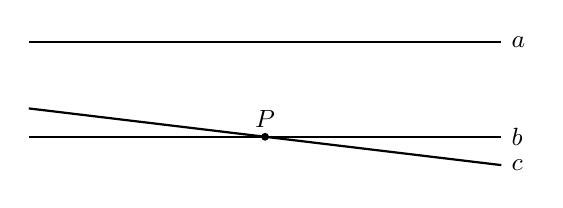
\begin{tikzpicture}[scale=1.2,font=\small, dot/.style={circle,inner sep=1pt, fill, label={#1}, name=#1}, extended line/.style={shorten >=-#1,shorten <=-#1}, extended line/.default=1cm]
\usetikzlibrary{calc, intersections}

\begin{scope}

\coordinate (a1) at (-2.5,0);
\coordinate (a2) at (2.5,0);
\coordinate (b1) at (-2.5,-1);
\coordinate (b2) at (2.5,-1);

\coordinate (c1) at (-2.5,-0.7);
\coordinate (c2) at (2.5,-1.3);

\draw[thick] (a1)--(a2) node[right] {$a$};
\draw[thick] (b1)--(b2) node[right] {$b$};
\draw[thick] (c1)--(c2) node[right] {$c$};

\coordinate (p) at (intersection of c1--c2 and b1--b2);
\draw[fill] (p) circle (1pt) node[above] {$P$};

\end{scope}


\end{tikzpicture}

\end{figure}
\end{inaccessibleblock}

\begin{proof}
Siano $a$, $b$, $c$ tre rette, con $a\parallel b$. Se $a$ coincide 
con $b$, la tesi è banale. Supponiamo quindi che $a$ e $b$ non 
abbiano punti in comune.
Vogliamo dimostrare che se $c\parallel a$ allora $c\parallel b$.
La tesi è banale se $c$ coincide con $a$ oppure con $b$.
Supponiamo dunque che $c$ sia distinta da entrambe.
Dimostriamo che se $c$ non ha punti in comune con $a$, allora non può 
avere punti in comune neppure con $b$. Se per assurdo $c$ avesse un 
punto $P$ in comune con $b$, allora esisterebbero due rette distinte 
passanti per $P$ entrambe parallele alla stessa retta $a$, cosa che 
contraddice il V postulato di Euclide.

Dimostriamo ora che se $c$ interseca la retta $a$ allora interseca 
anche la retta $b$. Detto $Q$ il punto di intersezione tra le rette 
$a$ e $c$, se per assurdo $c$ non intersecasse la retta $b$, cioè se 
fosse $c\parallel b$, allora $a$ e $c$ sarebbero due rette distinte 
passanti per $Q$ entrambe parallele alla retta $b$, contrariamente a 
quanto dice il V postulato di Euclide.
\end{proof}

\begin{osservazione}
La proposizione precedente rappresenta una sorta di proprietà 
transitiva del parallelismo. In realtà si è scelto di considerare 
parallele sia rette nel piano che non hanno punti in comune sia rette 
coincidenti proprio per fare in modo che la relazione di parallelismo 
sia una relazione di equivalenza: riflessiva, simmetrica, transitiva. 
Con la definizione di parallelismo data da Euclide, al contrario, 
sarebbe stata solo simmetrica, ma non riflessiva né transitiva. Per 
convincersi della non transitività, basta considerare tre rette $a$, 
$b$, $c$ con $a$ e $c$ coincidenti e $b$ parallela ad entrambe e 
distinta da esse: allora $a\parallel b$ e $b \parallel c$, ma $a$ e 
$c$ non sono parallele secondo la definizione di Euclide.
\end{osservazione}

\subsection{Rette parallele tagliate da una trasversale}

Due rette parallele $a$ e $b$ vengono intersecate da una retta $c$ 
(detta \emph{trasversale}) che non è parallela ad esse,
\begin{itemize*}
\item se la retta $c$ è perpendicolare (ad entrambe), si vengono a 
formare otto angoli retti; 
\item se la retta $c$ non è perpendicolare ad esse, si vengono a 
formare otto angoli, di cui quattro acuti e quattro ottusi, rispetto 
alla posizione che occupano alle coppie vengono attribuiti i seguenti 
nomi (figura~\ref{fig:rette_parall_2}):
\begin{itemize*}
\item le coppie di angoli 1 e 5, 2 e 6, 3 e 7, 4 e 8 si dicono 
\emph{corrispondenti} (perché occupano posizioni analoghe da una 
parallela all'altra);
\item le coppie di angoli 3 e 5, 4 e 6 si dicono \emph{alterni 
interni} (alterni perché occupano posizioni opposte rispetto alla 
trasversale, interni perché si trovano all'interno delle due 
parallele);
\item le coppie di angoli 1 e 7, 2 e 8 si dicono \emph{alterni 
esterni} (alterni perché sono opposti rispetto alla trasversale; 
esterni perché si trovano all'esterno della zona tra le due 
parallele);
\item le coppie di angoli 3 e 6, 4 e 5 si dicono \emph{coniugati 
interni} (si dicono coniugati perché stanno dalla stessa parte 
rispetto alla trasversale);
\item le coppie di angoli 1 e 8, 2 e 7 si dicono \emph{coniugati 
esterni}.
\end{itemize*}
\end{itemize*}
Inoltre le coppie 1 e 3, 2 e 4, 5 e 7, 6 e 8 sono angoli opposti al 
vertice.


\begin{inaccessibleblock}[Figura: TODO]
 \begin{figure}[htb]
\centering% Copyright (c) 2015 Daniele Masini - d.masini.it@gmail.com

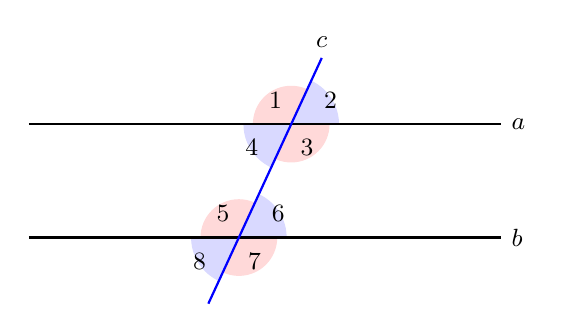
\begin{tikzpicture}[scale=1.2,font=\small, dot/.style={circle,inner sep=1pt, fill, label={#1}, name=#1}, extended line/.style={shorten >=-#1,shorten <=-#1}, extended line/.default=1cm]
\usetikzlibrary{calc, intersections}

\begin{scope}

\coordinate (a1) at (-2.5,0);
\coordinate (a2) at (2.5,0);
\coordinate (b1) at (-2.5,-1.2);
\coordinate (b2) at (2.5,-1.2);

\coordinate (c1) at (0.6,0.7);
\coordinate (c2) at (-0.6,-1.9);

\coordinate (p1) at (intersection of c1--c2 and a1--a2);
\coordinate (p2) at (intersection of c1--c2 and b1--b2);

\begin{scope}
\clip (a1) -- (p1) -- (c1) -- cycle;
\draw[fill, red!15] (p1) circle (0.4) node[shift={(-0.2,0.3)}, black] {1};
\end{scope}

\begin{scope}
\clip (a2) -- (p1) -- (c1) -- cycle;
\draw[fill, blue!15] (p1) circle (0.5) node[shift={(0.5,0.3)}, black] {2};
\end{scope}

\begin{scope}
\clip (a2) -- (p1) -- (c2) -- cycle;
\draw[fill, red!15] (p1) circle (0.4) node[shift={(0.2,-0.3)}, black] {3};
\end{scope}

\begin{scope}
\clip (a1) -- (p1) -- (c2) -- cycle;
\draw[fill, blue!15] (p1) circle (0.5) node[shift={(-0.5,-0.3)}, black] {4};
\end{scope}

\begin{scope}
\clip (b1) -- (p2) -- (c1) -- cycle;
\draw[fill, red!15] (p2) circle (0.4) node[shift={(-0.2,0.3)}, black] {5};
\end{scope}

\begin{scope}
\clip (b2) -- (p2) -- (c1) -- cycle;
\draw[fill, blue!15] (p2) circle (0.5) node[shift={(0.5,0.3)}, black] {6};
\end{scope}

\begin{scope}
\clip (b2) -- (p2) -- (c2) -- cycle;
\draw[fill, red!15] (p2) circle (0.4) node[shift={(0.2,-0.3)}, black] {7};
\end{scope}

\begin{scope}
\clip (b1) -- (p2) -- (c2) -- cycle;
\draw[fill, blue!15] (p2) circle (0.5) node[shift={(-0.5,-0.3)}, black] {8};
\end{scope}

\draw[thick] (a1)--(a2) node[right] {$a$};
\draw[thick] (b1)--(b2) node[right] {$b$};
\draw[thick, blue] (c1) node[above, black] {$c$} --(c2);

\end{scope}


\end{tikzpicture}

\caption{Le rette parallele $a$ e $b$ sono tagliate dalla trasversale 
$c$}\label{fig:rette_parall_2}
\end{figure}
\end{inaccessibleblock}

\begin{teorema}[delle parallele {[}diretto{]}]
Se due rette tagliate da una trasversale formano una coppia di angoli 
alterni interni congruenti allora sono parallele.
\end{teorema}


\begin{inaccessibleblock}[Figura: TODO]
 \begin{figure}[htb]
\centering% Copyright (c) 2015 Daniele Masini - d.masini.it@gmail.com

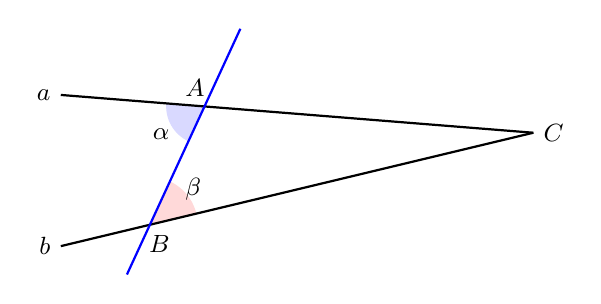
\begin{tikzpicture}[scale=1.2,font=\small, dot/.style={circle,inner sep=1pt, fill, label={#1}, name=#1}, extended line/.style={shorten >=-#1,shorten <=-#1}, extended line/.default=1cm]
\usetikzlibrary{calc, intersections}

\begin{scope}

\coordinate (a1) at (-2.5,0);
\coordinate (a2) at (2.5,-0.4);
\coordinate (b1) at (-2.5,-1.6);
\coordinate (b2) at (2.5,-0.4);

\coordinate (c1) at (-0.6,0.7);
\coordinate (c2) at (-1.8,-1.9);

\coordinate (p1) at (intersection of c1--c2 and a1--a2);
\coordinate (p2) at (intersection of c1--c2 and b1--b2);

\begin{scope}
\clip (a1) -- (p1) -- (c2) -- cycle;
\draw[fill, blue!15] (p1) circle (0.4) node[shift={(-0.55,-0.35)}, black] {$\alpha$};
\end{scope}

\begin{scope}
\clip (b2) -- (p2) -- (c1) -- cycle;
\draw[fill, red!15] (p2) circle (0.5) node[shift={(0.55,0.45)}, black] {$\beta$};
\end{scope}

\draw[thick] (a1) node[left] {$a$} --(a2) node[right] {$C$};
\draw[thick] (b1) node[left] {$b$}--(b2) ;
\draw[thick,blue] (c1) -- (c2);
\node at ([shift={(-0.1,0.2)}]p1) {$A$};
\node at ([shift={(0.1,-0.2)}]p2) {$B$};

\end{scope}


\end{tikzpicture}

\end{figure}
\end{inaccessibleblock}

\begin{proof}
Ragioniamo per assurdo. Supponiamo che la tesi sia falsa, cioè che le 
rette $a$ e $b$ non siano parallele. Se non sono parallele si 
incontreranno in un punto $C$ e quindi tra esse e la trasversale si 
viene a formare il triangolo $ABC$. Per il teorema dell'angolo 
esterno del triangolo, l'angolo (esterno) $\alpha$ è maggiore 
dell'angolo (interno) $\beta$. Questa conseguenza contraddice 
l'ipotesi del teorema, secondo la quale gli angoli alterni interni 
$\alpha$ e $\beta$ sono congruenti. Allora abbiamo sbagliato a negare 
la tesi, che perciò risulta vera.
\end{proof}

Possiamo generalizzare il teorema precedente ad altri casi.
\begin{teorema}[Criterio di parallelismo]
Se due rette tagliate da una trasversale danno origine ad una tra le 
seguenti coppie di angoli
\begin{itemize*}
\item angoli alterni interni o alterni esterni congruenti;
\item angoli corrispondenti congruenti;
\item angoli coniugati interni o coniugati esterni supplementari
\end{itemize*}
allora sono parallele.
\end{teorema}

\noindent \begin{minipage}{0.7\textwidth}
\begin{proof}
Tenendo conto che due angoli opposti al vertice sono congruenti e due 
angoli adiacenti sono supplementari, se risulta che due angoli 
corrispondenti qualsiasi sono congruenti, allora i quattro angoli 
acuti sono tutti congruenti ed i quattro angoli ottusi sono 
congruenti, e quindi anche angoli alterni interni. Pertanto, per il 
teorema precedente, le rette sono parallele.

\hspace{15pt}Analogamente, se risultano supplementari due qualsiasi 
angoli coniugati (interni o esterni) risulta sempre che i quattro 
angoli acuti sono tutti congruenti tra loro come i quattro angoli 
ottusi, pertanto gli angoli alterni interni sono congruenti e, sempre 
per il teorema precedente, le due rette sono parallele.
\end{proof}
\end{minipage}\hfil
\begin{minipage}{0.3\textwidth}
\centering% Copyright (c) 2015 Daniele Masini - d.masini.it@gmail.com

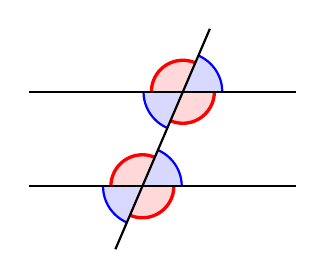
\begin{tikzpicture}[scale=1,font=\small, dot/.style={circle,inner sep=1pt, fill, label={#1}, name=#1}, extended line/.style={shorten >=-#1,shorten <=-#1}, extended line/.default=1cm]
\usetikzlibrary{calc, intersections}

\begin{scope}

\coordinate (a1) at (-1.7,0);
\coordinate (a2) at (1.7,0);
\coordinate (b1) at (-1.7,-1.2);
\coordinate (b2) at (1.7,-1.2);

\coordinate (c1) at (0.6,0.8);
\coordinate (c2) at (-0.6,-2);

\coordinate (p1) at (intersection of c1--c2 and a1--a2);
\coordinate (p2) at (intersection of c1--c2 and b1--b2);

\begin{scope}
\clip (a1) -- (p1) -- (c1) -- cycle;
\draw[very thick, red, fill=red!15] (p1) circle (0.4);
\end{scope}

\begin{scope}
\clip (a2) -- (p1) -- (c1) -- cycle;
\draw[thick, blue, fill=blue!15] (p1) circle (0.5);
\end{scope}

\begin{scope}
\clip (a2) -- (p1) -- (c2) -- cycle;
\draw[very thick, red, fill=red!15] (p1) circle (0.4);
\end{scope}

\begin{scope}
\clip (a1) -- (p1) -- (c2) -- cycle;
\draw[thick, blue, fill=blue!15] (p1) circle (0.5);
\end{scope}

\begin{scope}
\clip (b1) -- (p2) -- (c1) -- cycle;
\draw[very thick, red, fill=red!15] (p2) circle (0.4);
\end{scope}

\begin{scope}
\clip (b2) -- (p2) -- (c1) -- cycle;
\draw[thick, blue, fill=blue!15] (p2) circle (0.5);
\end{scope}

\begin{scope}
\clip (b2) -- (p2) -- (c2) -- cycle;
\draw[very thick, red, fill=red!15] (p2) circle (0.4);
\end{scope}

\begin{scope}
\clip (b1) -- (p2) -- (c2) -- cycle;
\draw[thick, blue, fill=blue!15] (p2) circle (0.5);
\end{scope}

\draw[thick] (a1)--(a2);
\draw[thick] (b1)--(b2);
\draw[thick] (c1) --(c2);

\end{scope}


\end{tikzpicture}

\end{minipage}

\begin{teorema}[delle parallele {[}inverso{]}]
Se due rette sono parallele allora esse formano con una trasversale 
qualsiasi due angoli alterni interni congruenti.
\end{teorema}

\noindent \begin{minipage}{0.6\textwidth}
\begin{proof}
Ragioniamo per assurdo. Supponiamo che la tesi sia falsa, cioè che 
esista una coppia di angoli alterni interni $\alpha$ e $\beta$ con 
$\alpha>\beta$. Per il punto $P$, vertice dell'angolo $\alpha$ si 
potrà allora tracciare una retta $a'$ in modo che l'angolo da essa 
formato $\alpha'$ sia congruente a $\beta$. Ne segue che $a'$ e $b$ 
sono parallele perché formano angoli alterni interni congruenti. 
Allora esisterebbero due rette distinte, $a$ e $a'$, passanti per lo 
stesso punto $P$, entrambe parallele alla retta $b$. Questa 
conclusione contraddice il V postulato di Euclide, secondo il quale 
per un punto esterno a una retta passa un'unica parallela. In altre 
parole la tesi è vera.
\end{proof}
\end{minipage}\hfil
\begin{minipage}{0.4\textwidth}
\centering% Copyright (c) 2015 Daniele Masini - d.masini.it@gmail.com

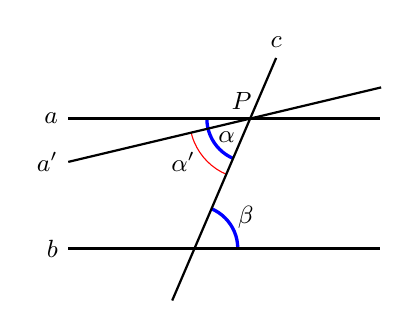
\begin{tikzpicture}[scale=1.1,font=\small, dot/.style={circle,inner sep=1pt, fill, label={#1}, name=#1}, extended line/.style={shorten >=-#1,shorten <=-#1}, extended line/.default=1cm]
\usetikzlibrary{calc, intersections}

\begin{scope}

\coordinate (a1) at (-1.8,0);
\coordinate (a2) at (1.8,0);
\coordinate (b1) at (-1.8,-1.5);
\coordinate (b2) at (1.8,-1.5);

\coordinate (aa1) at (-1.8,-0.5);

\coordinate (c1) at (0.6,0.7);
\coordinate (c2) at (-0.6,-2.1);

\coordinate (p1) at (intersection of c1--c2 and a1--a2);
\coordinate (p2) at (intersection of c1--c2 and b1--b2);


\begin{scope}
\clip (aa1) -- (p1) -- (c2) -- cycle;
\draw[red] (p1) circle (0.7) node[shift={(-0.85,-0.55)}, black] {$\alpha'$};
\end{scope}

\begin{scope}
\clip (a1) -- (p1) -- (c2) -- cycle;
\draw[blue, very thick] (p1) circle (0.5) node[shift={(-0.3,-0.23)}, black] {$\alpha$};
\end{scope}

\begin{scope}
\clip (b2) -- (p2) -- (c1) -- cycle;
\draw[blue, very thick] (p2) circle (0.5) node[shift={(0.65,0.4)}, black] {$\beta$};
\end{scope}


\draw[thick] (a1) node[left] {$a$} --(a2);
\draw[thick] (aa1) node[left] {$a'$} -- ($(aa1)!1.72!(p1)$);
\draw[thick] (b1) node[left] {$b$} --(b2);
\draw[thick] (c1) node[above] {$c$} --(c2);
\node at ([shift={(-0.1,0.2)}]p1) {$P$};

\end{scope}


\end{tikzpicture}

\end{minipage}
~\\

In generale possiamo enunciare il seguente
\begin{teorema}
Se due rette sono parallele allora esse formano con una trasversale 
qualunque
\begin{itemize*}
\item angoli alterni interni o alterni esterni congruenti;
\item angoli corrispondenti congruenti;
\item angoli coniugati interni o coniugati esterni supplementari.
\end{itemize*}
\end{teorema}

\begin{proof}
Abbiamo già dimostrato che sono congruenti gli angoli alterni interni 
formati da due parallele tagliate da una trasversale. Tenendo conto 
che gli angoli opposti al vertice sono congruenti e gli angoli 
adiacenti sono supplementari, si possono dedurre facilmente tutte le 
tesi di questo teorema.
\end{proof}


\section{Somma degli angoli interni di un 
triangolo}\label{sect:angoli_interni_triangolo}

Passiamo ora a dimostrare il secondo teorema dell'angolo esterno di 
un triangolo.
\begin{teorema}
In un triangolo, un angolo esterno è congruente alla somma dei due 
angoli interni non adiacenti.
\end{teorema}


\begin{inaccessibleblock}[Figura: TODO]
 \begin{figure}[htb]
\centering% Copyright (c) 2015 Daniele Masini - d.masini.it@gmail.com

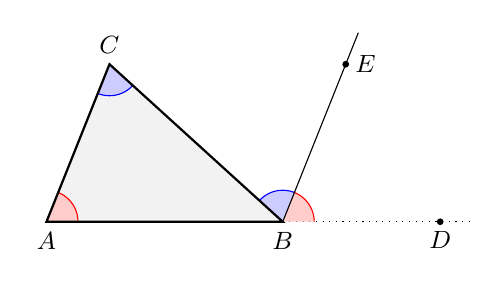
\begin{tikzpicture}[scale=1,font=\small, dot/.style={circle,inner sep=1pt, fill, label={#1}, name=#1}, extended line/.style={shorten >=-#1,shorten <=-#1}, extended line/.default=1cm]
\usetikzlibrary{calc, intersections}

\begin{scope}

\coordinate (a) at (0,0);
\coordinate (b) at (3,0);
\coordinate (c) at (0.8,2);
\coordinate (d) at (5,0);
\coordinate (e) at (3.8,2);

\draw[fill, gray!10] (a) node[below] {$A$} -- (b) node[below] {$B$} -- (c) node[above] {$C$} -- cycle;
\draw[dotted] (b) -- ($(b)!1.2!(d)$);
\draw[fill] (d) circle (1pt) node[below] {$D$};

\begin{scope}
\clip (a) -- (b) -- (c) -- cycle;
\draw[red,fill=red!20] (a) circle (0.4) node[shift={(-0.85,-0.55)}, black] {$\alpha'$};
\draw[blue,fill=blue!20] (c) circle (0.4) node[shift={(-0.85,-0.55)}, black] {$\alpha'$};
\end{scope}

\begin{scope}
\clip (b) -- (e) -- (d) -- cycle;
\draw[red,fill=red!20] (b) circle (0.4) node[shift={(-0.85,-0.55)}, black] {$\alpha'$};
\end{scope}
\begin{scope}
\clip (b) -- (c) -- (e) -- cycle;
\draw[blue,fill=blue!20] (b) circle (0.4) node[shift={(-0.85,-0.55)}, black] {$\alpha'$};
\end{scope}

\draw[fill] (e) circle (1pt) node[right] {$E$};
\draw (b) -- ($(b)!1.2!(e)$);
\draw[thick] (a) node[below] {$A$} -- (b) node[below] {$B$} -- (c) node[above] {$C$} -- cycle;

\end{scope}


\end{tikzpicture}

\end{figure}
\end{inaccessibleblock}

\begin{proof}
Sia $ABC$ un triangolo e sia $C\widehat{B}D$ un angolo esterno. 
Tracciamo la semiretta $BE\parallel AC$ che divide l'angolo 
$C\widehat{B}D$ in due parti, $C\widehat{B}E$ ed $E\widehat{B}D$. 
L'angolo $C\widehat{B}E$ risulta congruente all'angolo 
$A\widehat{C}B$ in quanto i due angoli sono alterni interni rispetto 
alle rette parallele $AC$ e $BE$ tagliate dalla trasversale $CB$; 
analogamente l'angolo $E\widehat{B}D$ risulta congruente all'angolo 
$C\widehat{A}B$ in quanto i due angoli sono corrispondenti rispetto 
alle rette parallele $AC$ e $BE$ tagliate dalla trasversale $AD$. 
Dunque $C\widehat{B}D$ è congruente alla somma degli angoli interni 
di vertici $A$ e $C$.
\end{proof}

\begin{corollario}
La somma degli angoli interni di un triangolo è congruente ad un 
angolo piatto.
\end{corollario}
\begin{proof}
Dalla figura precedente $A\widehat{B}D\cong A\widehat{B}C + 
C\widehat{B}E + E\widehat{B}D\cong A\widehat{B}C + B\widehat{C}A + 
C\widehat{A}B$, pertanto la somma degli angoli interni è congruente 
all'angolo piatto $A\widehat{B}D$.
\end{proof}
\begin{corollario}
Un triangolo non può avere più di un angolo retto e/o ottuso.
\end{corollario}
Dunque, necessariamente almeno due angoli sono acuti. Di conseguenza, 
gli angoli alla base di un triangolo isoscele devono essere acuti.

\section{Somma degli angoli interni di un 
poligono}\label{sect:angoli_interni_poligono}

\begin{teorema}
Dato un poligono $P$ di $n$ lati, la somma degli angoli interni di 
$P$ è $n-2$ angoli piatti.
\end{teorema}
\noindent \begin{minipage}{0.5\textwidth}
\begin{proof}
Infatti, dato un qualunque poligono (anche concavo) di $n$ lati, 
scelto un opportuno punto interno $J$ in modo che, congiunto con esso 
ciascun vertice il poligono resti diviso in $n$ triangoli, si può 
osservare che la somma degli angoli interni del poligono è data dalla 
somma degli angoli interni di $n$ triangoli ($n$ angoli piatti) meno 
l'angolo giro (2 angoli piatti) in $J$.
\end{proof}
\end{minipage}\hfil
\begin{minipage}{0.5\textwidth}
\centering% Copyright (c) 2015 Daniele Masini - d.masini.it@gmail.com

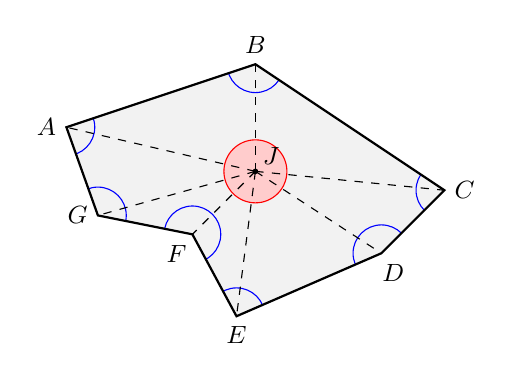
\begin{tikzpicture}[scale=0.8,font=\small, dot/.style={circle,inner sep=1pt, fill, label={#1}, name=#1}, extended line/.style={shorten >=-#1,shorten <=-#1}, extended line/.default=1cm]
\usetikzlibrary{calc, intersections}

\begin{scope}

\coordinate (a) at (0,0);
\coordinate (b) at (3,1);
\coordinate (c) at (6,-1);
\coordinate (d) at (5,-2);
\coordinate (e) at (2.7,-3);
\coordinate (f) at (2,-1.7);
\coordinate (g) at (0.5,-1.4);
\coordinate (j) at (3,-0.7);

\draw[fill, gray!10] (a) -- (b) -- (c) -- (d) -- (e) -- (f) -- (g) -- cycle;
\draw[red, fill=red!20] (j) circle (0.5);

\begin{scope}
\clip (a) -- (b) -- (c) -- (d) -- (e) -- (f) -- (g) -- cycle;
\draw[blue] (a) circle (0.45);
\draw[blue] (b) circle (0.45);
\draw[blue] (c) circle (0.45);
\draw[blue] (d) circle (0.45);
\draw[blue] (e) circle (0.45);
\draw[blue] (f) circle (0.45);
\draw[blue] (g) circle (0.45);
\end{scope}

\draw[fill] (j) circle (1pt) node[shift={(0.2,0.2)}] {$J$};
\draw[dashed] (j) -- (a);
\draw[dashed] (j) -- (b);
\draw[dashed] (j) -- (c);
\draw[dashed] (j) -- (d);
\draw[dashed] (j) -- (e);
\draw[dashed] (j) -- (f);
\draw[dashed] (j) -- (g);

\draw[thick] (a) node[left] {$A$} -- (b) node[above] {$B$} -- (c) node[right] {$C$} -- (d) node[shift={(0.15,-0.25)}] {$D$} -- (e) node[below] {$E$} -- (f) node[shift={(-0.2,-0.25)}] {$F$} -- (g) node[left] {$G$} -- cycle;

\end{scope}


\end{tikzpicture}

\end{minipage}

\begin{teorema}
La somma degli angoli esterni di un qualsiasi poligono convesso, 
indipendentemente dal numero dei lati, è congruente ad un angolo giro.
\end{teorema}
\noindent \begin{minipage}{0.5\textwidth}
\begin{proof}
Ogni angolo esterno è adiacente ad un angolo interno, per cui se si 
hanno $m$ lati, e quindi $m$ vertici, la somma degli angoli interni e 
degli angoli esterni è pari ad $m$ angoli piatti. Essendo la somma 
degli angoli interni congruente a $m-2$ angoli piatti (per il teorema 
precedente), la somma degli angoli esterni sarà di due angoli piatti, 
cioè un angolo giro.
\end{proof}
\end{minipage}\hfil
\begin{minipage}{0.5\textwidth}
\centering% Copyright (c) 2015 Daniele Masini - d.masini.it@gmail.com

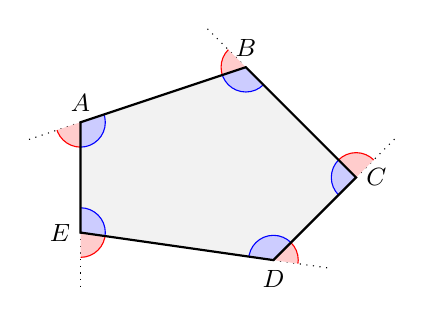
\begin{tikzpicture}[scale=0.7,font=\small, dot/.style={circle,inner sep=1pt, fill, label={#1}, name=#1}, extended line/.style={shorten >=-#1,shorten <=-#1}, extended line/.default=1cm]
\usetikzlibrary{calc, intersections}

\begin{scope}

\coordinate (a) at (0,0);
\coordinate (b) at (3,1);
\coordinate (c) at (5,-1);
\coordinate (d) at (3.5,-2.5);
\coordinate (e) at (0,-2);
\coordinate (f) at (2.4,-0.7);

\draw[fill, gray!10] (a) -- (b) -- (c) -- (d) -- (e) -- cycle;
%\draw[red, fill=red!20] (f) circle (0.5);

\begin{scope}
\clip (a) -- (b) -- (c) -- (d) -- (e) -- cycle;
\draw[blue, fill=blue!20] (a) circle (0.45);
\draw[blue, fill=blue!20] (b) circle (0.45);
\draw[blue, fill=blue!20] (c) circle (0.45);
\draw[blue, fill=blue!20] (d) circle (0.45);
\draw[blue, fill=blue!20] (e) circle (0.45);
\end{scope}

\draw[dotted] (a) -- ($(a)!-1cm!(b)$) coordinate (a1);
\draw[dotted] (b) -- ($(b)!-1cm!(c)$) coordinate (b1);
\draw[dotted] (c) -- ($(c)!-1cm!(d)$) coordinate (c1);
\draw[dotted] (d) -- ($(d)!-1cm!(e)$) coordinate (d1);
\draw[dotted] (e) -- ($(e)!-1cm!(a)$) coordinate (e1);

\begin{scope}
\clip (a) -- (e) -- (a1) -- cycle;
\draw[red, fill=red!20] (a) circle (0.45);
\end{scope}
\begin{scope}
\clip (b) -- (a) -- (b1) -- cycle;
\draw[red, fill=red!20] (b) circle (0.45);
\end{scope}
\begin{scope}
\clip (c) -- (b) -- (c1) -- cycle;
\draw[red, fill=red!20] (c) circle (0.45);
\end{scope}
\begin{scope}
\clip (d) -- (c) -- (d1) -- cycle;
\draw[red, fill=red!20] (d) circle (0.45);
\end{scope}
\begin{scope}
\clip (e) -- (d) -- (e1) -- cycle;
\draw[red, fill=red!20] (e) circle (0.45);
\end{scope}

%\draw[fill] (f) circle (1pt) node[below] {$F$};
%\draw[dashed] (f) -- (a);
%\draw[dashed] (f) -- (b);
%\draw[dashed] (f) -- (c);
%\draw[dashed] (f) -- (d);
%\draw[dashed] (f) -- (e);

\draw[thick] (a) node[above] {$A$} -- (b) node[above] {$B$} -- (c) node[right] {$C$} -- (d) node[below] {$D$} -- (e) node[left] {$E$} -- cycle;

\end{scope}


\end{tikzpicture}

\end{minipage}


\section{Generalizzazione dei criteri di congruenza dei 
triangoli}\label{sect:generalizzazione_criteri_congruenza_triangoli}

Se due triangoli hanno rispettivamente due angoli congruenti, allora 
anche i terzi angoli saranno congruenti nei due triangoli, in quanto 
supplementari della somma di angoli congruenti.

Dunque, se due triangoli hanno congruenti un lato e due angoli, anche 
se il lato congruente non è compreso tra i due angoli congruenti, 
risultano congruenti. Precisamente, vale la seguente proposizione.

\begin{teorema}[Generalizzazione del 2\textsuperscript{o} criterio di 
congruenza dei triangoli]
Due triangoli sono congruenti se hanno rispettivamente congruenti una 
coppia di lati e due coppie di angoli ugualmente posti rispetto ai 
lati congruenti.
\end{teorema}


\begin{inaccessibleblock}[Figura: TODO]
 \begin{figure}[htb]
\centering% Copyright (c) 2015 Daniele Masini - d.masini.it@gmail.com

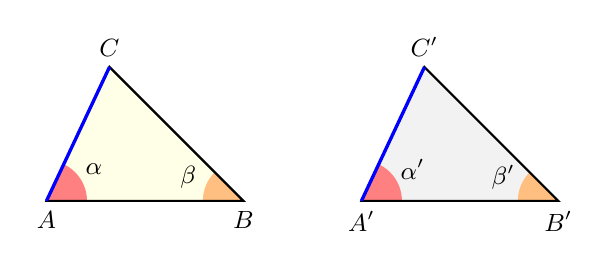
\begin{tikzpicture}[scale=1,font=\small]
\usetikzlibrary{calc}

\begin{scope}
\coordinate (a) at (0,0);
\coordinate (c) at (0.8,1.7);
\coordinate (b) at (2.5,0);
\draw[fill=yellow!10] (a) -- (b) -- (c) -- cycle;

\begin{scope}
\clip (a) -- (b) -- (c) -- cycle;
\draw[thick,red!50,fill] (a) circle (0.5);
\node at ([shift={(0.6,0.4)}]a) {$\alpha$};
\draw[thick,orange!50,fill] (b) circle (0.5);
\node at ([shift={(-0.7,0.3)}]b) {$\beta$};
\end{scope}

\draw[thick] (a) node[below] {$A$} -- (b) node[below] {$B$} -- (c) node[above] {$C$} -- cycle;
\draw[blue,very thick] (a) -- (c);


\end{scope}

\begin{scope}[xshift=4cm]
\coordinate (a) at (0,0);
\coordinate (c) at (0.8,1.7);
\coordinate (b) at (2.5,0);
\draw[fill=gray!10] (a) -- (b) -- (c) -- cycle;

\begin{scope}
\clip (a) -- (b) -- (c) -- cycle;
\draw[thick,red!50,fill] (a) circle (0.5);
\node at ([shift={(0.65,0.4)}]a) {$\alpha'$};
\draw[thick,orange!50,fill] (b) circle (0.5);
\node at ([shift={(-0.7,0.3)}]b) {$\beta'$};
\end{scope}

\draw[thick] (a) node[below] {$A'$} -- (b) node[below] {$B'$} -- (c) node[above] {$C'$} -- cycle;
\draw[blue,very thick] (a) -- (c);

\end{scope}

\end{tikzpicture}

\end{figure}
\end{inaccessibleblock}

\begin{proof}
Il caso in cui il lato congruente è compreso tra gli angoli 
congruenti è stato già dimostrato (2\textsuperscript{o} criterio di 
congruenza dei triangoli) ed utilizzato per la dimostrazione di varie 
proprietà. Ora consideriamo l'altro caso.

In figura abbiamo rappresentato due triangoli, $ABC$ e $A'B'C'$ che 
hanno per ipotesi i lati $AC\cong A'C'$ e gli angoli $\alpha\cong 
\alpha'$ e $\beta\cong \beta'$. I due triangoli risultano congruenti, 
poiché deve risultare $A\widehat{C}B\cong A'\widehat{C'}B'$, in 
quanto tali angoli sono supplementari alla somma di angoli congruenti 
per ipotesi (la somma degli angoli interni di un triangolo è un 
angolo piatto). Ci riconduciamo quindi al caso del 
2\textsuperscript{o} criterio di congruenza, già dimostrato in 
precedenza.
\end{proof}

Riprendiamo una proprietà dei triangoli isosceli che abbiamo 
enunciato ma non abbiamo dimostrato.
\begin{proposizione}
In un triangolo isoscele, l'altezza relativa alla base è anche 
bisettrice dell'angolo al vertice e mediana relativa alla base.
\end{proposizione}

\noindent \begin{minipage}{0.6\textwidth}
\noindent Ipotesi: $IG\cong IH$, $\alpha\cong \beta$, $IL\perp GH$.\\
Tesi: $G\widehat{I}L\cong H\widehat{I}L$, $GL\cong LH$.

\begin{proof}
I triangoli $GLI$ e $LHI$ sono congruenti per il secondo criterio 
generalizzato, avendo congruenti un lato (quello obliquo, $IG\cong 
IH$) e due angoli ($\alpha\cong \beta$ e $I\widehat{L}G \cong 
I\widehat{L}H$). Di conseguenza, i restanti elementi sono 
ordinatamente congruenti, in particolare $GL\cong LH$ e 
$G\widehat{I}L\cong H\widehat{I}L$.
\end{proof}
\end{minipage}\hfil
\begin{minipage}{0.4\textwidth}
\centering% Copyright (c) 2015 Daniele Masini - d.masini.it@gmail.com

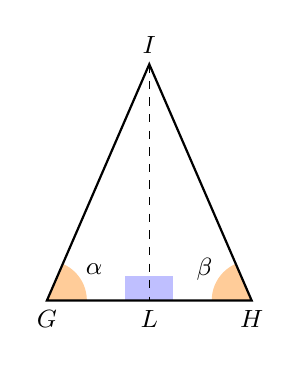
\begin{tikzpicture}[scale=1,font=\small]
\usetikzlibrary{calc}

\begin{scope}
\coordinate (a) at (-1.3,0);
\coordinate (b) at (1.3,0);
\coordinate (c) at (0,3);
\coordinate (j) at (0,0);

\begin{scope}
\clip (a) -- (b) -- (c) -- cycle;
\draw[fill,orange!40] (a) circle (0.5);
\draw[fill,orange!40] (b) circle (0.5);
\node at ([shift={(0.6,0.4)}]a) {$\alpha$};
\node at ([shift={(-0.6,0.4)}]b) {$\beta$};
\coordinate (j1) at ($(j)!0.3cm!(b)$);
\draw[fill,blue!25] ($(j)!0.3cm!(a)$) rectangle ($(j1)!0.3cm!90:(b)$);
\end{scope}

\draw[dashed] (c) -- (j) node[below] {$L$};
\draw[thick] (a) node[below] {$G$} -- (b) node[below] {$H$} -- (c) node[above] {$I$} -- cycle;

\end{scope}

\end{tikzpicture}

\end{minipage}

\osservazione Dall'esame dei primi tre criteri di congruenza dei 
triangoli, nonché dalla generalizzazione del secondo criterio, si 
potrebbe essere indotti a pensare che due triangoli sono congruenti 
se hanno tre coppie di elementi rispettivamente congruenti, se almeno 
una delle tre coppie di elementi è costituita da lati.

\noindent \begin{minipage}{0.6\textwidth}
In realtà, il primo criterio non si può generalizzare come il 
secondo. Basta pensare alla figura a lato: $ADC$ è un triangolo 
isoscele, $B$ è un punto sul prolungamento della base $AD$. Unendo $B$ 
con $C$, vengono individuati due nuovi triangoli, $ABC$ e $BCD$ che 
hanno in comune il lato $CB$ e l'angolo di vertice $B$, ed hanno 
inoltre congruenti i lati $AC$ e $CD$, ma evidentemente non sono 
congruenti. Quindi se due triangoli hanno due lati ed un angolo 
qualsiasi congruenti, non è detto che siano congruenti. Però nei due 
triangoli citati in figura, gli angoli $C\widehat{A}B$ e 
$C\widehat{D}B$ sono supplementari.
\end{minipage}\hfil
\begin{minipage}{0.4\textwidth}
\centering% Copyright (c) 2015 Daniele Masini - d.masini.it@gmail.com

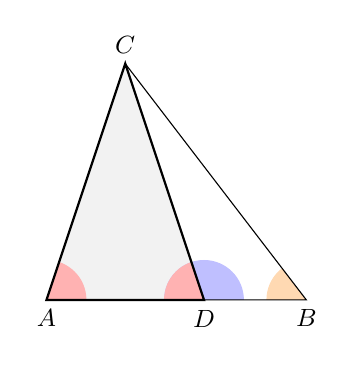
\begin{tikzpicture}[scale=1,font=\small]
\usetikzlibrary{calc}

\begin{scope}
\coordinate (a) at (-1,0);
\coordinate (b) at (2.3,0);
\coordinate (c) at (0,3);
\coordinate (d) at (1,0);

\coordinate (j) at (0,0);

\draw[fill, gray!10] (a) -- (d) -- (c) -- cycle;

\begin{scope}
\clip (a) -- (b) -- (c) -- cycle;
\draw[fill,red!30] (a) circle (0.5);
\draw[fill,orange!30] (b) circle (0.5);
%\node at ([shift={(0.6,0.4)}]a) {$\alpha$};
%\node at ([shift={(-0.6,0.4)}]b) {$\beta$};
\draw[fill,blue!25] (d) circle (0.5);
\end{scope}

\begin{scope}
\clip (a) -- (d) -- (c) -- cycle;
\draw[fill,red!30] (d) circle (0.5);
\end{scope}

\draw[thick] (a) -- (c) -- (d) node[below] {$D$} -- cycle;
\draw (a) node[below] {$A$} -- (b) node[below] {$B$} -- (c) node[above] {$C$} -- cycle;

\end{scope}

\end{tikzpicture}

\end{minipage}

Tale osservazione fa da premessa al 4\textsuperscript{o} criterio di 
congruenza dei triangoli.
\begin{teorema}[4\textsuperscript{o} criterio di congruenza dei 
triangoli]
Due triangoli sono congruenti se hanno congruenti due coppie di lati 
e l'angolo opposto ad uno di essi, a patto che l'angolo opposto 
all'altra coppia di lati congruenti sia della stessa specie (cioè 
sia, in entrambi i triangoli, acuto, retto, oppure ottuso).
\end{teorema}

\noindent Ipotesi: $AC\cong DF$, $CB\cong FE$, $\alpha\cong \beta$, 
$C\widehat{B}A$ e $F\widehat{E}D$ della stessa specie.\tab Tesi: 
$ABC\cong DEF$.


\begin{inaccessibleblock}[Figura: TODO]
 \begin{figure}[htb]
\centering% Copyright (c) 2015 Daniele Masini - d.masini.it@gmail.com

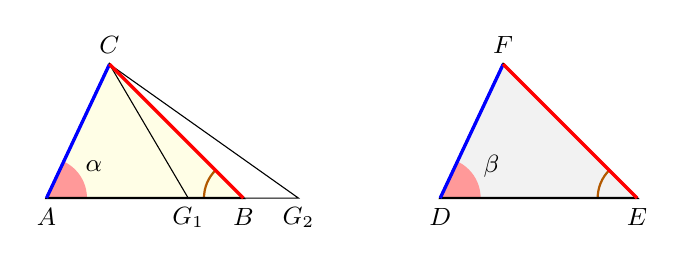
\begin{tikzpicture}[scale=1,font=\small]
\usetikzlibrary{calc}

\begin{scope}
\coordinate (a) at (0,0);
\coordinate (c) at (0.8,1.7);
\coordinate (b) at (2.5,0);
\draw[fill=yellow!10] (a) -- (b) -- (c) -- cycle;
\coordinate (g1) at (1.8,0);
\coordinate (g2) at (3.2,0);

\begin{scope}
\clip (a) -- (b) -- (c) -- cycle;
\draw[thick,red!40,fill] (a) circle (0.5);
\node at ([shift={(0.6,0.4)}]a) {$\alpha$};
\draw[thick,orange!70!black] (b) circle (0.5);
%\node at ([shift={(-0.7,0.3)}]b) {$\beta$};
\end{scope}

\draw (c) -- (g1) node[below] {$G_1$};
\draw (c) -- (g2) node[below] {$G_2$} -- (b);

\draw[thick] (a) node[below] {$A$} -- (b) node[below] {$B$} -- (c) node[above] {$C$} -- cycle;
\draw[blue,very thick] (a) -- (c);
\draw[red,very thick] (c) -- (b);

\end{scope}

\begin{scope}[xshift=5cm]
\coordinate (a) at (0,0);
\coordinate (c) at (0.8,1.7);
\coordinate (b) at (2.5,0);
\draw[fill=gray!10] (a) -- (b) -- (c) -- cycle;

\begin{scope}
\clip (a) -- (b) -- (c) -- cycle;
\draw[thick,red!40,fill] (a) circle (0.5);
\node at ([shift={(0.65,0.4)}]a) {$\beta$};
\draw[thick,orange!70!black] (b) circle (0.5);
%\node at ([shift={(-0.7,0.3)}]b) {$\beta'$};
\end{scope}

\draw[thick] (a) node[below] {$D$} -- (b) node[below] {$E$} -- (c) node[above] {$F$} -- cycle;
\draw[blue,very thick] (a) -- (c);
\draw[red,very thick] (c) -- (b);

\end{scope}

\end{tikzpicture}

\end{figure}
\end{inaccessibleblock}

\begin{proof}
Sulla semiretta $AB$ prendiamo il punto $G$ in maniera tale che $AG$ 
sia congruente a $DE$. I triangoli $AGC$ e $DEF$ saranno congruenti 
per il primo criterio, poiché $AC\cong DF$ e $\alpha\cong \beta$ per 
ipotesi e $AG\cong DE$ per costruzione. Di conseguenza anche i 
rimanenti elementi risulteranno congruenti, in particolare $CG\cong 
FE$ e $C\widehat{G}A\cong F\widehat{E}D$.

Se il punto $G$ coincide con $B$, abbiamo dimostrato la congruenza 
dei triangoli $ABC$ e $DEF$. Altrimenti, il segmento $CG$, dovendo 
essere congruente ad $FE$, risulta congruente a $CB$. Dunque il 
triangolo $CGB$ è isoscele sulla base $GB$ e quindi gli angoli alla 
base $C\widehat{G}B$ e $C\widehat{B}G$, congruenti, sono 
necessariamente acuti. Distinguiamo due casi:
\begin{itemize*}
\item se $G$ è interno al segmento $AB$ ($G_1$ nella figura), 
$C\widehat{G}B$ è esterno al triangolo $AGC$ e $C\widehat{B}G$ è 
interno al triangolo $ABC$, quindi $D\widehat{E}F\cong A\widehat{G}C$ 
ottuso e $A\widehat{B}C$ acuto;
\item se $G$ è esterno al segmento $AB$ ($G_2$ nella figura), 
$C\widehat{G}B$ è interno al triangolo $AGC$ e $C\widehat{B}G$ è 
esterno al triangolo $ABC$, quindi $D\widehat{E}F\cong A\widehat{G}C$ 
acuto e $A\widehat{B}C$ ottuso.
\end{itemize*}
Dunque, in nessuno dei due casi viene rispettata l'ipotesi, quindi 
$C\widehat{B}A$ e $F\widehat{E}D$ sono della stessa specie.
\end{proof}

\subsection{Congruenze di triangoli rettangoli}

Per quanto affermato nelle proposizioni precedenti, sappiamo che i 
triangoli rettangoli hanno una coppia di angoli congruenti (quelli 
retti, essendo tutti congruenti fra loro, come affermato dal IV 
postulato di Euclide) e gli altri angoli necessariamente acuti, in 
quanto la somma degli angoli interni di un triangolo è congruente ad 
un angolo piatto (come segue dal secondo teorema dell'angolo esterno 
e dai corollari).

Tenendo conto dunque dei criteri di congruenza dei triangoli, si 
possono riformulare dei criteri di congruenza specifici per i 
triangoli rettangoli.

\begin{teorema}[Criteri di congruenza dei triangoli rettangoli]
Due triangoli rettangoli sono congruenti se hanno rispettivamente 
congruenti almeno uno tra:
\begin{itemize*}
\item i due cateti (1\textsuperscript{o} criterio);
\item l'ipotenusa e un angolo acuto (2\textsuperscript{o} criterio);
\item un cateto e l'angolo acuto adiacente (2\textsuperscript{o} 
criterio);
\item un cateto e l'angolo acuto opposto (2\textsuperscript{o} 
criterio);
\item un cateto e l'ipotenusa (4\textsuperscript{o} criterio).
\end{itemize*}
\end{teorema}

L'ultimo criterio dell'elenco è detto anche \emph{criterio 
particolare di congruenza dei triangoli rettangoli} (ha naturalmente 
una formulazione più semplice del 4\textsuperscript{o} criterio di 
congruenza dei triangoli perché si sa già che le coppie di angoli non 
citati nell'ipotesi sono ``della stessa specie'', perché certamente 
acuti). Due triangoli rettangoli che hanno congruenti l'ipotenusa ed 
un cateto hanno congruenti due coppie di lati e l'angolo opposto ad 
uno di essi (l'angolo retto, opposto all'ipotenusa), ed hanno gli 
angoli opposti all'altra coppia di lati congruenti della stessa 
specie (gli angoli opposti ai cateti congruenti sono acuti in entrambi 
i triangoli). 

Data l'importanza di tale criterio, nonché la sua semplice 
dimostrazione, indipendente dal quarto criterio di congruenza dei 
triangoli qualunque, lo riformuliamo a parte e ne proponiamo una 
dimostrazione:
\begin{teorema}[Criterio particolare di congruenza dei triangoli 
rettangoli]
Due triangoli rettangoli sono congruenti se hanno ordinatamente 
congruenti un cateto e l'ipotenusa.
\end{teorema}

\noindent Ipotesi: $C\widehat{A}B\cong C'\widehat{A'}B'$ retto, 
$AC\cong A'C'$, $BC\cong B'C'$.\tab\tab Tesi: $ABC\cong A'B'C'$.


\begin{inaccessibleblock}[Figura: TODO]
 \begin{figure}[htb]
\centering% Copyright (c) 2015 Daniele Masini - d.masini.it@gmail.com

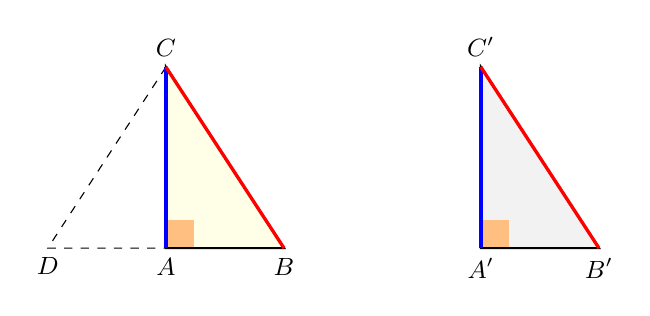
\begin{tikzpicture}[scale=1,font=\small]
\usetikzlibrary{calc}

\begin{scope}
\coordinate (a) at (0,0);
\coordinate (c) at (0,2.3);
\coordinate (b) at (1.5,0);
\draw[fill=yellow!10] (a) -- (b) -- (c) -- cycle;
\coordinate (b1) at (-1.5,0);

\draw[fill,orange!50] (a) rectangle ([shift={(0.35,0.35)}]a);
\draw[dashed] (c) -- (b1) node[below] {$D$} -- (b);

\draw[thick] (a) node[below] {$A$} -- (b) node[below] {$B$} -- (c) node[above] {$C$} -- cycle;
\draw[blue,very thick] (a) -- (c);
\draw[red,very thick] (c) -- (b);

\end{scope}

\begin{scope}[xshift=4cm]
\coordinate (a) at (0,0);
\coordinate (c) at (0,2.3);
\coordinate (b) at (1.5,0);
\draw[fill=gray!10] (a) -- (b) -- (c) -- cycle;

\draw[fill,orange!50] (a) rectangle ([shift={(0.35,0.35)}]a);

\draw[thick] (a) node[below] {$A'$} -- (b) node[below] {$B'$} -- (c) node[above] {$C'$} -- cycle;
\draw[blue,very thick] (a) -- (c);
\draw[red,very thick] (c) -- (b);

\end{scope}

\end{tikzpicture}

\end{figure}
\end{inaccessibleblock}

\begin{proof}
Si prolunga il cateto $AB$ di un segmento $AD$ congruente ad $A'B'$, 
quindi si congiunge $D$ con $C$. Il triangolo $ADC$ è anch'esso 
rettangolo in $A$, in quanto l'angolo $D\widehat{A}C$ è adiacente ad 
un angolo retto ($C\widehat{A}B$). I triangoli rettangoli $ADC$ e 
$A'B'C'$ sono congruenti per il primo criterio, in quanto hanno i due 
cateti ordinatamente congruenti: $AC\cong A'C'$ per ipotesi e 
$AB\cong A'B'$ per costruzione. Di conseguenza risulterà $CB\cong 
C'B'$ e dunque $CD\cong CB$ (per la proprietà transitiva della 
congruenza, essendo $CB\cong C'B'$ per ipotesi). Quindi il triangolo 
$DCB$ è isoscele sulla base $DB$, e di conseguenza, per il teorema 
(diretto) del triangolo isoscele, i suoi angoli alla base sono 
congruenti: $A\widehat{B}C\cong A\widehat{D}C$.

Allora i triangoli $ABC$ e $A'B'C'$ sono congruenti per il secondo 
criterio generalizzato, avendo ordinatamente congruenti due coppie di 
angoli e il lato opposto ad uno di essi (l'ipotenusa).
\end{proof}

\section{Disuguaglianze tra gli elementi di un 
triangolo}\label{sect:disuguaglianze_triangoli}

\begin{teorema}
In un triangolo, a lato maggiore si oppone angolo maggiore.
\end{teorema}

\noindent\begin{minipage}{0.7\textwidth}
\noindent Ipotesi: $BC>AB$. Tesi: $B\widehat{A}C>A\widehat{C}B$.

\begin{proof}
Scegliamo opportunamente un punto $D$ sul lato maggiore $BC$ in modo 
che $BD$ sia congruente ad $AB$. Se uniamo $A$ con $D$, poiché il 
segmento $AD$ è interno al triangolo $ABC$, il triangolo $ABC$ viene 
diviso in due nuovi triangoli, $ADB$ e $ACD$. Il triangolo $ADB$ è 
isoscele sulla base $AD$ pertanto ha gli angoli alla base congruenti, 
per cui risulta $B\widehat{A}D\cong A\widehat{D}B$. Ma 
$B\widehat{A}D$ è una parte propria di $B\widehat{A}C$, mentre 
$A\widehat{D}B$, come angolo esterno al triangolo $ACD$ è maggiore 
dell'angolo $A\widehat{C}D=A\widehat{C}B$, interno non adiacente, per 
il primo teorema dell'angolo esterno. Si ha dunque: 
$B\widehat{A}C>B\widehat{A}D\cong A\widehat{D}B>A\widehat{C}B$ e 
quindi la tesi (in maniera del tutto analoga si può dimostrare che 
$B\widehat{A}C>A\widehat{B}C$).
\end{proof}
\end{minipage}\hfil
\begin{minipage}{0.3\textwidth}
\centering% Copyright (c) 2015 Daniele Masini - d.masini.it@gmail.com

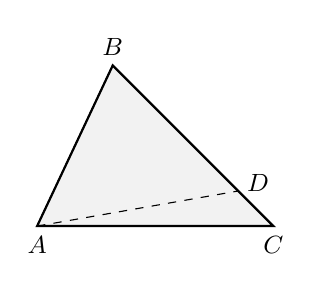
\begin{tikzpicture}[scale=1.2,font=\small]
\usetikzlibrary{calc, through, intersections}

\begin{scope}
\clip (-0.1,-0.5) rectangle (2.6,2.1);
\coordinate (a) at (0,0);
\coordinate (b) at (0.8,1.7);
\coordinate (c) at (2.5,0);
\draw[fill=gray!10] (a) -- (b) -- (c) -- cycle;

\node (c1) at (b) [circle through={(a)}] {};
\coordinate(d) at (intersection 1 of c1 and b--c);

\draw[dashed] (a) -- (d) node[shift={(0.25,0.1)}] {$D$};

\draw[thick] (a) node[below] {$A$} -- (b) node[above] {$B$} -- (c) node[below] {$C$} -- cycle;

\end{scope}

\end{tikzpicture}

\end{minipage}

\begin{teorema}
In un triangolo, ad angolo maggiore si oppone lato maggiore.
\end{teorema}

\noindent\begin{minipage}{0.7\textwidth}\parindent15pt 
\noindent Ipotesi: $B\widehat{A}C>A\widehat{C}B$. Tesi: $BC>AB$.

\noindent\begin{proof}
\noindent Dimostriamo la tesi in maniera indiretta, facendo uso del 
teorema precedente e del teorema del triangolo isoscele. Supponiamo 
vera l'ipotesi $B\widehat{A}C>A\widehat{C}B$. Facciamo un confronto 
tra i segmenti $BC$ e $AB$ considerando tutte le possibilità. \`E 
possibile che sia:
\[\text{(i) }BC\cong AB\text{;}\qquad\qquad \text{(ii) 
}BC<AB\text{;}\quad\quad\text{(iii) }BC>AB\text{.}\]

Se fosse vera la (i), il triangolo $ABC$ sarebbe isoscele sulla base 
$AC$ e risulterebbe $B\widehat{A}C\cong A\widehat{C}B$, per il 
teorema del triangolo isoscele, contro l'ipotesi.

Se fosse vera la (ii), per il teorema precedente risulterebbe 
$B\widehat{A}C<A\widehat{C}B$, contro l'ipotesi.

Rimane solo la possibilità che sia vera la (iii), la quale infatti 
non contraddice il teorema precedente, anzi lo conferma. Quindi la 
tesi è dimostrata.
\end{proof}
\end{minipage}\hfil
\begin{minipage}{0.3\textwidth}
\centering% Copyright (c) 2015 Daniele Masini - d.masini.it@gmail.com

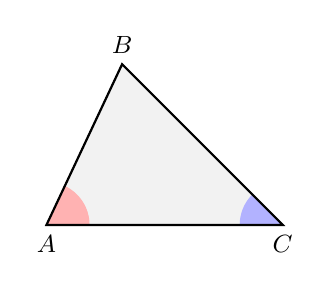
\begin{tikzpicture}[scale=1.2,font=\small]
\usetikzlibrary{calc, through, intersections}

\begin{scope}
\coordinate (a) at (0,0);
\coordinate (b) at (0.8,1.7);
\coordinate (c) at (2.5,0);
\draw[fill=gray!10] (a) -- (b) -- (c) -- cycle;

\begin{scope}
\clip (a) -- (b) -- (c);
\draw[fill, red!30] (a) circle (0.45);
\draw[fill, blue!30] (c) circle (0.45);
\end{scope}

\draw[thick] (a) node[below] {$A$} -- (b) node[above] {$B$} -- (c) node[below] {$C$} -- cycle;

\end{scope}

\end{tikzpicture}

\end{minipage}
~\\

Da questo teorema discende la proprietà che in un triangolo 
rettangolo l'ipotenusa è sempre maggiore di ciascuno dei due cateti, 
in quanto l'ipotenusa è il lato che si oppone all'angolo maggiore, 
l'angolo retto.

Ora dimostriamo una proprietà importante dei triangoli, nota come 
\emph{disuguaglianza triangolare}.

\begin{teorema}[Disuguaglianza triangolare]
In un triangolo, ciascun lato è minore della somma degli altri due e 
maggiore della loro differenza.
\end{teorema}

\noindent\begin{minipage}{0.7\textwidth}\parindent15pt 
\begin{proof}
In riferimento alla figura a lato, dimostriamo che nel triangolo 
$ABC$, $AC < AB + BC$. Se $AC$ fosse minore di un altro lato, 
sicuramente sarebbe minore della somma degli altri due e il teorema 
sarebbe dimostrato. Esaminiamo il caso in cui $AC$ è maggiore sia di 
$AB$ che di $BC$. Prolunghiamo il lato $AB$ dalla parte di $B$ e 
prendiamo un punto $D$ sul prolungamento in modo che il segmento $BD$ 
sia congruente a $BC$. Unendo $D$ con $C$ abbiamo il triangolo $ACD$ 
nel quale il lato $AD$ è congruente alla somma dei lati $AB$ e $BC$. 
La tesi si riconduce dunque a dimostrare che il lato $AC$ è minore di 
$AD$. Osserviamo che il triangolo $CBD$ è isoscele sulla base $CD$, 
per cui i suoi angoli alla base sono congruenti: $B\widehat{C}D\cong 
B\widehat{D}C$. Ma l'angolo $B\widehat{C}D$ è una parte propria di 
$A\widehat{C}D$ che quindi risulta maggiore di $B\widehat{C}D\cong 
A\widehat{D}C$. Dunque, nel triangolo $ACD$, il lato $AD$, che si 
oppone ad angolo maggiore, è maggiore del lato $AC$, che si oppone ad 
angolo minore, per il teorema precedente.
 
Visto che la costruzione fatta si può ripetere tale e quale rispetto 
a qualsiasi lato, si può concludere che $AC<AB+BC$, $AB<AC+BC$, 
$BC<AB+AC$ e dunque, sottraendo ad ambo i membri della prima 
disuguaglianza il lato $BC$ si ha $AC-AB<BC$, analogamente, 
sottraendo uno stesso segmento, si hanno $AC-BC<AB$, $AC-BC<AB$, 
$AB-AC<BC$, $AB-BC<AC$, $BC-AC<AB$, $BC-AB<AC$. Leggendo le relazioni 
da destra verso sinistra, ogni lato è maggiore della differenza degli 
altri due (abbiamo scritto tutte le disuguaglianze, anche se 
ovviamente ogni lato ha misura positiva mentre la differenza tra due 
lati può essere anche nulla o negativa).
\end{proof}
\end{minipage}\hfil
\begin{minipage}{0.3\textwidth}
\centering% Copyright (c) 2015 Daniele Masini - d.masini.it@gmail.com

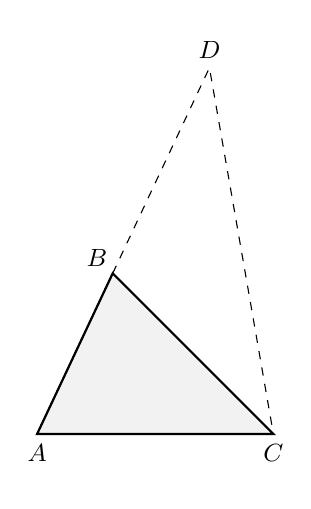
\begin{tikzpicture}[scale=1.2,font=\small]
\usetikzlibrary{calc, through, intersections}

\begin{scope}
\clip (-0.1,-0.5) rectangle (2.6,4.3);
\coordinate (a) at (0,0);
\coordinate (b) at (0.8,1.7);
\coordinate (c) at (2.5,0);
\draw[fill=gray!10] (a) -- (b) -- (c) -- cycle;

\node (c1) at (b) [circle through={(c)}] {};
\coordinate(d) at (intersection 1 of c1 and a--b);

\draw[dashed] (b) -- (d) node[above] {$D$} -- (c);

\draw[thick] (a) node[below] {$A$} -- (b) node[shift={(-0.2,0.2)}] {$B$} -- (c) node[below] {$C$} -- cycle;

\end{scope}

\end{tikzpicture}

\end{minipage}

Proponiamo ora un teorema sulle disuguaglianze tra gli elementi di 
due triangoli.

Supponiamo di avere due triangoli aventi due coppie di lati 
rispettivamente congruenti. Allora, se anche gli angoli compresi sono 
congruenti, i due triangoli risultano congruenti per il primo 
criterio. Altrimenti, se i due angoli compresi tra i lati congruenti 
non sono congruenti, i due triangoli non sono congruenti, ed i terzi 
lati sono diseguali nello stesso verso degli angoli opposti ad essi 
(cioè compresi tra i lati congruenti).

\begin{teorema}
Se due lati di un triangolo sono rispettivamente congruenti a due 
lati di un altro triangolo, e l'angolo tra essi compreso è nel primo 
triangolo maggiore che nel secondo, allora il terzo lato del primo 
triangolo è maggiore del terzo lato del secondo.
\end{teorema}

\noindent Ipotesi: $AB\cong DE$, $AC\cong DF$, 
$B\widehat{A}C>E\widehat{D}F$ ($AB\leq AC$). Tesi: $BC>EF$.


\begin{inaccessibleblock}[Figura: TODO]
 \begin{figure}[htb]
\centering% Copyright (c) 2015 Daniele Masini - d.masini.it@gmail.com

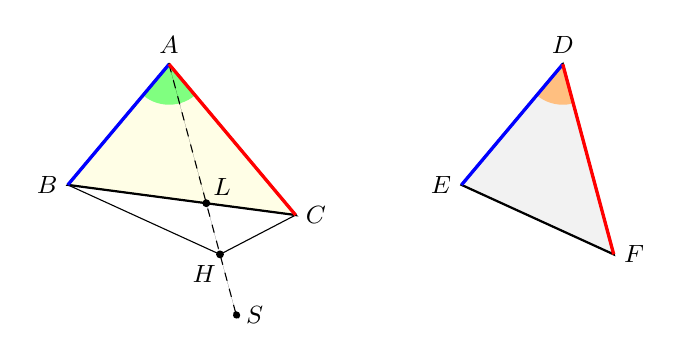
\begin{tikzpicture}[scale=1,font=\small]
\usetikzlibrary{calc}

\begin{scope}

\draw[fill=yellow!10] (0,0) coordinate (b) -- ++(50:2) coordinate (a) -- ++(-50:2.5) coordinate (c) -- cycle;

\begin{scope}
\clip (a) -- (b) -- (c) -- cycle;
\draw[thick,green!50,fill] (a) circle (0.5);
%\node at ([shift={(0.65,0.4)}]a) {$\beta$};
\end{scope}

\draw[fill,dashed] (a) -- ++(-75:3.3) circle (1.2pt) coordinate (s) node[right] {$S$};
\draw[fill] ($(a)!{2.5/3.3}!(s)$) circle (1.2pt) coordinate (h) node[shift={(-0.2,-0.25)}] {$H$};
\draw (h) -- (b);

\coordinate (l) at (intersection of a--s and b--c);
\draw[fill] (l) circle (1.2pt) node[shift={(0.2,0.2)}] {$L$};
\draw (h) -- (c);

\draw[thick] (a) node[above] {$A$} -- (b) node[left] {$B$} -- (c) node[right] {$C$} -- cycle;
\draw[blue,very thick] (a) -- (b);
\draw[red,very thick] (a) -- (c);

\end{scope}

\begin{scope}[xshift=5cm]

\draw[fill=gray!10] (0,0) coordinate (b) -- ++(50:2) coordinate (a) -- ++(-75:2.5) coordinate (c) -- cycle;

\begin{scope}
\clip (a) -- (b) -- (c) -- cycle;
\draw[thick,orange!50,fill] (a) circle (0.5);
%\node at ([shift={(0.65,0.4)}]a) {$\beta$};
\end{scope}

\draw[thick] (a) node[above] {$D$} -- (b) node[left] {$E$} -- (c) node[right] {$F$} -- cycle;
\draw[blue,very thick] (a) -- (b);
\draw[red,very thick] (a) -- (c);

\end{scope}

\end{tikzpicture}

\end{figure}
\end{inaccessibleblock}

\begin{proof}
Tracciamo la semiretta $AS$ di origine $A$, interna all'angolo 
$B\widehat{A}C$, in modo tale che $B\widehat{A}S\cong E\widehat{D}F$. 
Se prendiamo su $AS$ il punto $H$ tale che $AH\cong DF$ ed uniamo $H$ 
con $B$, otteniamo un triangolo $ABH$ congruente a $DEF$ per il primo 
criterio.

\`E importante dimostrare che il punto $H$ è esterno al triangolo 
$ABC$. Per dimostrare ciò, prendiamo il punto $L$, intersezione tra 
la semiretta $AS$ ed il lato $BC$. Notiamo che abbiamo iniziato la 
costruzione a partire dal lato $AB$ avendo supposto $AB\leq AC$, ma 
da questa disuguaglianza segue la corrispondente disuguaglianza tra 
gli angoli opposti: $A\widehat{B}C\geq A\widehat{C}B$. L'angolo 
$A\widehat{L}C$ è esterno al triangolo $ABL$, pertanto è maggiore 
dell'angolo $A\widehat{B}C$ per il primo teorema dell'angolo esterno. 
Mettendo insieme le due disuguaglianze si ha 
$A\widehat{L}C>A\widehat{B}C\geq A\widehat{C}B$, dunque nel triangolo 
$ALC$ vale la seguente relazione tra due angoli: 
$A\widehat{L}C>A\widehat{C}B$. Vale quindi anche la corrispondente 
relazione tra i lati opposti, per cui $AC>AL$. Poiché $AX\cong 
DF\cong AC$, il punto $L$ è interno al segmento $AH$, e dunque $H$ è 
esterno al triangolo $ABC$.

Abbiamo già unito $H$ con $B$, uniamo $H$ anche con $C$ e ragioniamo 
sul triangolo $BHC$. Essendo $BH$ congruente ad $EF$, la tesi è 
ricondotta a dimostrare che $BC$ è maggiore di $BH$. Confrontiamo i 
rispettivi angoli opposti. Poiché il triangolo $AHC$ è isoscele sulla 
base $HC$, gli angoli alla base risultano congruenti 
$A\widehat{H}C\cong A\widehat{C}H$, dunque risulta 
$B\widehat{H}C\cong B\widehat{C}H$ perché:
\[B\widehat{H}C=B\widehat{H}A+A\widehat{H}C>A\widehat{H}C\cong 
A\widehat{C}H=A\widehat{C}B+B\widehat{C}H>B\widehat{C}H.\]
Dalla precedente disuguaglianza tra gli angoli segue la 
corrispondente disuguaglianza tra i lati opposti $BC>BH$ e dunque la 
tesi.
\end{proof}

\begin{teorema}
Se due lati di un triangolo sono, rispettivamente, congruenti a due 
lati di un altro triangolo, e il terzo lato del primo triangolo è 
maggiore del terzo lato del secondo, allora l'angolo opposto al lato 
diseguale (compreso tra i lati congruenti) è nel primo triangolo 
maggiore che nel secondo.
\end{teorema}

\noindent Ipotesi: $AB\cong DE$, $AC\cong DF$, $BC>EF$. Tesi: 
$B\widehat{A}C>E\widehat{D}F$.


\begin{inaccessibleblock}[Figura: TODO]
 \begin{figure}[htb]
\centering% Copyright (c) 2015 Daniele Masini - d.masini.it@gmail.com

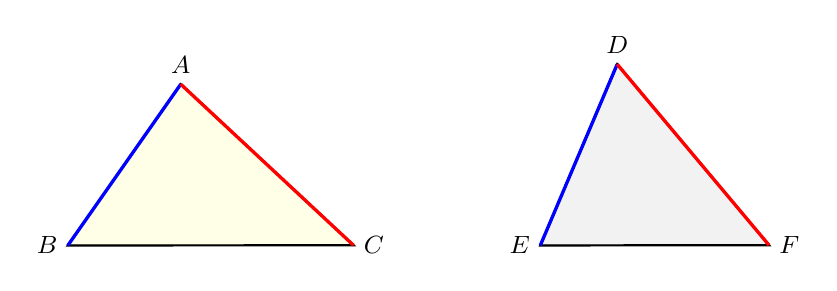
\begin{tikzpicture}[scale=1,font=\small]
\usetikzlibrary{calc}

\begin{scope}

\draw[fill=yellow!10] (0,0) coordinate (b) -- ++(55:2.5) coordinate (a) -- ++(-43:3) coordinate (c) -- cycle;

\draw[thick] (a) node[above] {$A$} -- (b) node[left] {$B$} -- (c) node[right] {$C$} -- cycle;
\draw[blue,very thick] (a) -- (b);
\draw[red,very thick] (a) -- (c);

\end{scope}

\begin{scope}[xshift=6cm]

\draw[fill=gray!10] (0,0) coordinate (b) -- ++(67:2.5) coordinate (a) -- ++(-50:3) coordinate (c) -- cycle;

\draw[thick] (a) node[above] {$D$} -- (b) node[left] {$E$} -- (c) node[right] {$F$} -- cycle;
\draw[blue,very thick] (a) -- (b);
\draw[red,very thick] (a) -- (c);

\end{scope}

\end{tikzpicture}

\end{figure}
\end{inaccessibleblock}

\begin{proof}
Procediamo per esclusione, in maniera analoga a come abbiamo fatto 
nel teorema inverso sulle disuguaglianze tra gli elementi di un 
triangolo.

Supponiamo vera l'ipotesi e studiamo i vari casi delle possibili 
relazioni tra gli angoli citati nella tesi. Sono possibili tre casi:
\[\text{(i) }B\widehat{A}C\cong E\widehat{D}F\text{;}\qquad\qquad 
\text{(ii) }B\widehat{A}C<E\widehat{D}F\text{;}\qquad\qquad 
\text{(iii) }B\widehat{A}C>E\widehat{D}F\text{.}\]

Se valesse l'ipotesi (i), essendo anche $AB\cong DE$ e $AC\cong DF$, 
i triangoli risulterebbero congruenti per il primo criterio, 
contrariamente all'ipotesi $BC>EF$.

Se valesse l'ipotesi (ii), essendo anche $AB\cong DE$ e $AC\cong DF$, 
per il teorema precedente risulterebbe $BC<EF$, contrariamente 
all'ipotesi $BC>EF$.

Rimane l'ipotesi (iii), che non contraddice il teorema precedente e 
che anzi lo conferma. Dunque la tesi è dimostrata.
\end{proof}

Dalla disuguaglianza triangolare seguono alcune proprietà riguardanti 
i lati di poligoni.

\begin{teorema}
In un qualsiasi poligono, ciascun lato è minore della somma dei 
rimanenti.
\end{teorema}

\noindent\begin{minipage}{0.65\textwidth}\parindent15pt 
Nel quadrilatero $ABCD$ a fianco, se vogliamo dimostrare ad esempio 
che il lato $AD$ è minore della somma degli altri tre, tracciamo la 
diagonale $AC$ che divide il quadrilatero in due triangoli. Risulta 
$AD<AC+CD$, ed anche $AC<AB+BC$, per la disuguaglianza triangolare, 
per cui $AD<AB+BC+CD$.

Ma la proprietà non è limitata ai quadrilateri. Nel pentagono $EFGHI$ 
a fianco, se vogliamo dimostrare ad esempio che il lato $EI$ è minore 
della somma degli altri quattro, possiamo tracciare la diagonale $EG$ 
che divide il pentagono in un quadrilatero ed un triangolo. Se 
supponiamo che la tesi sia vera per i quadrilateri, verifichiamo che 
la tesi vale anche per i pentagoni. Infatti risulta $EI<EG+GH+HI$, in 
quanto la tesi è vera per i quadrilateri, e $EG<EF+FG$, per la 
disuguaglianza triangolare. Dunque $EI<EF+FG+GH+HI$, come volevasi 
dimostrare.\vspace{4pt}
\end{minipage}\hfil
\begin{minipage}{0.35\textwidth}
\centering% Copyright (c) 2015 Daniele Masini - d.masini.it@gmail.com

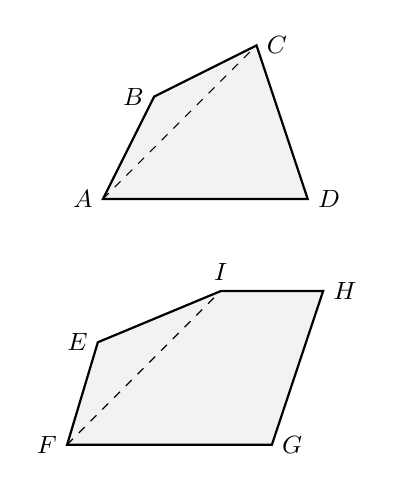
\begin{tikzpicture}[scale=1.3,font=\small]
\usetikzlibrary{calc}

\begin{scope}

\coordinate (a) at (0,0);
\coordinate (b) at (0.5,1);
\coordinate (c) at (1.5,1.5);
\coordinate (d) at (2,0);

\draw[fill, gray!10] (a) -- (b) -- (c) -- (d) -- cycle;
\draw[dashed] (a) -- (c);

\draw[thick] (a) node[left] {$A$} -- (b) node[left] {$B$} -- (c) node[right] {$C$} -- (d) node[right] {$D$} -- cycle;

\end{scope}

\begin{scope}[xshift=-0.35cm, yshift=-2.4cm]

\coordinate (e) at (0.3,1);
\coordinate (f) at (0,0);
\coordinate (g) at (2,0);
\coordinate (h) at (2.5,1.5);
\coordinate (i) at (1.5,1.5);

\draw[fill, gray!10] (e) -- (f) -- (g) -- (h) -- (i) -- cycle;
\draw[dashed] (f) -- (i);

\draw[thick] (e) node[left] {$E$} -- (f) node[left] {$F$} -- (g) node[right] {$G$} -- (h) node[right] {$H$} -- (i) node[above] {$I$} -- cycle;

\end{scope}

\end{tikzpicture}

\end{minipage}

In realtà, il passaggio che abbiamo fatto dai quadrilateri ai 
pentagoni vale anche per passare dai pentagoni agli esagoni ecc. 
seguendo il procedimento per induzione.
Più precisamente, poiché vale la disuguaglianza triangolare, la tesi 
è vera per i triangoli. Supponendo la tesi vera per tutti i poligoni 
di $n$~lati (con~$n\geq 3$) si dimostra che la tesi vale anche per i 
poligoni di $n+1$~lati. Allora, la tesi è vera per tutti i poligoni 
(aventi un numero qualsiasi di lati).

\begin{definizione}
Un poligono convesso si dice \emph{inscritto} in un altro se ogni 
vertice del primo giace sul contorno del secondo. Il secondo poligono 
è detto \emph{circoscritto} al primo.
\end{definizione}

\begin{teorema}
Se un poligono convesso è inscritto in un altro, il perimetro del 
primo è minore di quello del secondo.
\end{teorema}

Illustriamo con un semplice esempio il contenuto del teorema. Non è 
da escludere il caso che un lato del primo poligono giaccia 
interamente su un lato del secondo (e nemmeno che la stessa situazione 
valga per più lati), però è semplice dimostrare la disuguaglianza 
anche senza considerare le parti del contorno perfettamente 
sovrapposte.

\noindent\begin{minipage}{0.6\textwidth}\parindent15pt 
Osserviamo i quadrilateri $EFGH$ e $ABCD$ (il primo inscritto nel 
secondo) in figura; per la disuguaglianza triangolare $EF<EB+BF$, 
$FG<FC+CG$, $GH<GD+DH$, $HE<HA+AE$. La somma dei primi membri delle 
quattro disuguaglianze rappresenta il perimetro di $EFGH$, la somma 
dei secondi membri rappresenta il perimetro di $ABCD$.

La tesi del teorema precedente vale anche se il poligono, anziché 
essere inscritto, è semplicemente contenuto nell'altro. 
Illustriamo questa proprietà con un semplice esempio: il poligono 
$NOPQR$ è contenuto in $IJKLM$. Il lato $RQ$ è minore di $RS+SQ$ per 
la disuguaglianza triangolare. Dunque il perimetro del poligono 
$NOPQR$ è minore del perimetro di $NOPQS$, e quest'ultimo poligono è 
inscritto in $IJKLM$, per cui il perimetro di $NOPQS$ è minore del 
perimetro di $IJKLM$. Dalle due disuguaglianze segue la 
tesi.\vspace{4pt}
\end{minipage}\hfil
\begin{minipage}{0.4\textwidth}
\centering% Copyright (c) 2015 Daniele Masini - d.masini.it@gmail.com

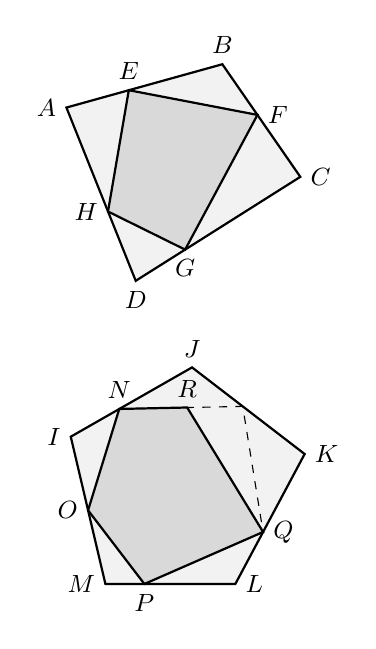
\begin{tikzpicture}[scale=1.1,font=\small]
\usetikzlibrary{calc}

\begin{scope}

\coordinate (a) at (-0.8,2);
\coordinate (b) at (1,2.5);
\coordinate (c) at (1.9,1.2);
\coordinate (d) at (0,0);

\draw[fill, gray!10] (a) -- (b) -- (c) -- (d) -- cycle;

\draw[fill, gray!30] ($(a)!0.4!(b)$) coordinate (e) -- ($(b)!0.45!(c)$) coordinate (f) -- ($(c)!0.7!(d)$) coordinate (g) -- ($(d)!0.4!(a)$) coordinate (h) -- cycle;

\draw[thick] (a) node[left] {$A$} -- (b) node[above] {$B$} -- (c) node[right] {$C$} -- (d) node[below] {$D$} -- cycle;
\draw[thick] (e) node[above] {$E$} -- (f) node[right] {$F$} -- (g) node[below] {$G$} -- (h) node[left] {$H$} -- cycle;

\end{scope}

\begin{scope}[xshift=-0.35cm, yshift=-3.5cm]

\coordinate (m) at (0,0);
\coordinate (i) at (-.4,1.7);
\coordinate (j) at (1,2.5);
\coordinate (k) at (2.3,1.5);
\coordinate (l) at (1.5,0);

\draw[fill, gray!10] (i) -- (j) -- (k) -- (l) -- (m) -- cycle;

\draw[dashed] ($(i)!0.4!(j)$) coordinate (n) -- ($(j)!0.45!(k)$) coordinate (s) -- ($(k)!0.6!(l)$) coordinate (q) -- ($(l)!0.7!(m)$) coordinate (p) -- ($(m)!0.5!(i)$) coordinate (o) -- cycle;

\coordinate (r) at ($(n)!0.55!(s)$);
\draw[thick,fill=gray!30] (n) node[above] {$N$} -- (o) node[left] {$O$} -- (p) node[below] {$P$} -- (q) node[right] {$Q$} -- (r) node[above] {$R$} -- cycle;

\draw[thick] (i) node[left] {$I$} -- (j) node[above] {$J$} -- (k) node[right] {$K$} -- (l) node[right] {$L$} -- (m) node[left] {$M$} -- cycle;

\end{scope}

\end{tikzpicture}

\end{minipage}

\begin{exrig}
\begin{esempio}
Nel triangolo $ABC$, isoscele sulla base $BC$, sia $D$ un punto 
qualsiasi sul lato $AB$. Dimostra che $DC>DB$.

\noindent\begin{minipage}{0.7\textwidth}\parindent15pt
\vspace{10pt}
\noindent Individuiamo ipotesi, tesi e costruiamo il 
disegno.\vspace{7pt}

\noindent Ipotesi: $AB\cong AC$, $D\in AB$.\tab Tesi: $CD>BD$.

\noindent\begin{proof}
Consideriamo i triangoli $ABC$ e $DBC$ a lato.\\
Poiché $B\widehat{C}D<B\widehat{C}A$ e $B\widehat{C}A\cong 
A\widehat{B}C$ si ha che $B\widehat{C}D<D\widehat{B}C$.
Quindi, poiché in un triangolo ad angolo maggiore si oppone lato 
maggiore, considerando il triangolo $DBC$ si ha $CD>BD$.
\end{proof}
\end{minipage}\hfil
\begin{minipage}{0.3\textwidth}
\centering% Copyright (c) 2015 Daniele Masini - d.masini.it@gmail.com

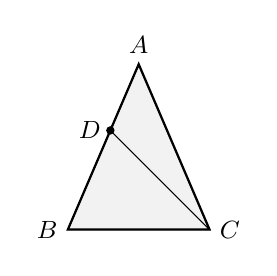
\begin{tikzpicture}[scale=1,font=\small]
\usetikzlibrary{calc, through, intersections}

\begin{scope}
\coordinate (a) at (0,0);
\coordinate (b) at (-0.9,-2.1);
\coordinate (c) at (0.9,-2.1);
\draw[fill=gray!10] (a) -- (b) -- (c) -- cycle;

\draw (c) -- ($(a)!0.4!(b)$) coordinate (d) node[left] {$D$};
\draw[fill] (d) circle (1.3pt);
\draw[thick] (a) node[above] {$A$} -- (b) node[left] {$B$} -- (c) node[right] {$C$} -- cycle;

\end{scope}

\end{tikzpicture}

\end{minipage}
\end{esempio}
\end{exrig}

% \newpage
% 
% \input{./chap/03_esercizi}
% 
% \cleardoublepage
